\documentclass[12pt,a4paper]{article}
\usepackage[margin=1in]{geometry}
\usepackage{amsmath}
\usepackage{amssymb}
\usepackage{amsthm}
\usepackage{graphicx}
\usepackage{cite}
\usepackage{url}
\usepackage{hyperref}
\usepackage{tikz}
\usepackage{pgfplots}
\usepackage{algorithm}
\usepackage{algorithmic}
\usepackage{subfigure}
\usepackage{multicol}
\usepackage{fancyhdr}

\pagestyle{fancy}
\fancyhf{}
\rhead{Universal Problem Reduction: A Theoretical Framework}
\lhead{Page \thepage}

\theoremstyle{definition}
\newtheorem{definition}{Definition}[section]
\newtheorem{theorem}{Theorem}[section]
\newtheorem{lemma}{Lemma}[section]
\newtheorem{proposition}{Proposition}[section]
\newtheorem{corollary}{Corollary}[section]
\newtheorem{example}{Example}[section]
\newtheorem{remark}{Remark}[section]

\title{Universal Problem Reduction: A Theoretical Framework for Computational Complexity Under Specific Architectural Constraints}

\author{Anonymous}

\date{\today}

\begin{document}

\maketitle

\begin{abstract}
This paper presents a theoretical framework that explores the possibility of reducing computational complexity under specific architectural constraints. The framework suggests that certain problem classes might be solvable within unit time bounds under highly specialized conditions involving biological quantum computing substrates, oscillatory processing paradigms, and recursive temporal precision enhancement. We examine the mathematical foundations that could potentially support such claims, while acknowledging the speculative nature of many components. The work is presented as a theoretical exploration rather than a practical implementation, with the understanding that significant gaps remain between theory and realizability. Key concepts include oscillatory-computational equivalence, biological quantum coherence preservation, and exponential parallel processing architectures. All results should be interpreted within the context of idealized mathematical models rather than physical implementations.
\end{abstract}

\section{Introduction}

The study of computational complexity has long been constrained by fundamental physical and mathematical limits that appear to establish inviolable boundaries on what can be computed within finite time and space. Classical complexity theory, rooted in the foundational work of Turing, Church, and subsequent theoretical computer scientists, establishes lower bounds on computational problems based on resource constraints including time, space, and energy \cite{arora2009computational}. These constraints have been further refined through decades of research into the fundamental limits of computation, including Landauer's principle regarding the thermodynamic cost of information processing \cite{landauer1961irreversibility} and the ultimate physical limits proposed by Lloyd \cite{lloyd2000ultimate}.

However, recent developments in quantum computing, biological information processing, and novel computational paradigms suggest that these constraints might be circumvented under specific architectural conditions. The emergence of quantum computing has already demonstrated that certain computational problems, such as integer factorization and unstructured search, can be solved exponentially faster than their classical counterparts \cite{shor1994algorithms, grover1996fast}. Similarly, investigations into biological information processing have revealed computational strategies that appear to transcend classical limitations through quantum coherence effects \cite{lambert2013quantum, huelga2013vibrations}.

This paper presents a theoretical framework that explores whether certain computational problems might be reducible to unit time complexity under highly specialized conditions involving what we term "biological quantum computing substrates," "oscillatory processing paradigms," and "recursive temporal precision enhancement." The framework is built upon several interconnected theoretical constructs that, while individually having some basis in established science, collectively represent a speculative synthesis that requires careful scrutiny and rigorous mathematical analysis.

The central thesis examines whether the equivalence between oscillatory systems and computational processors, combined with biological quantum coherence preservation and exponential recursive enhancement, might theoretically enable universal problem reduction. This represents a significant departure from established computational complexity theory, which generally assumes that certain problem classes are inherently intractable. We emphasize that this work is purely theoretical and does not claim practical realizability of the proposed systems without extensive experimental validation.

\subsection{Historical Context and Motivation}

The search for computational speedup has been a driving force in theoretical computer science since its inception. Early work by von Neumann and Turing established the theoretical foundations of computation, while subsequent researchers have continuously sought to push the boundaries of what is computationally feasible. The development of parallel computing, quantum computing, and other paradigms represents attempts to transcend classical limitations.

The motivation for this work stems from several observations:

\begin{enumerate}
\item \textbf{Quantum Biological Effects}: Recent experimental evidence suggests that biological systems may utilize quantum coherence for computational advantage in processes such as photosynthesis and avian navigation \cite{scholes2011lessons, ritz2000resonance}. These findings challenge the assumption that quantum effects are necessarily destroyed by the warm, noisy environment of biological systems.

\item \textbf{Oscillatory Universality}: Mathematical analysis of nonlinear dynamical systems reveals that virtually all finite systems exhibit oscillatory behavior under appropriate conditions \cite{strogatz1994nonlinear}. This universality suggests that oscillatory dynamics might serve as a fundamental computational substrate.

\item \textbf{Recursive Enhancement}: The observation that certain computational strategies can achieve exponential improvement through recursive application suggests that similar principles might apply to temporal precision and processing speed.

\item \textbf{Architectural Transcendence}: The history of computing demonstrates that architectural innovations can sometimes transcend apparent fundamental limits, as seen in the transition from mechanical to electronic to quantum computing paradigms.
\end{enumerate}

\subsection{Theoretical Foundations}

The framework presented in this paper rests on several theoretical pillars:

\subsubsection{Oscillatory-Computational Equivalence}

We propose that oscillatory systems and computational processors are mathematically equivalent under certain conditions. This equivalence is based on the observation that both systems involve the transformation of input states to output states through deterministic processes. In oscillatory systems, this transformation is mediated by dynamical evolution, while in computational systems, it is mediated by algorithmic operations.

The mathematical formalization of this equivalence requires careful analysis of the information-processing capabilities of oscillatory systems. We demonstrate that oscillatory systems can encode, manipulate, and decode information in ways that are functionally equivalent to traditional computational operations, potentially with significant advantages in terms of processing speed and energy efficiency.

\subsubsection{Biological Quantum Coherence}

The preservation of quantum coherence in biological systems represents a central challenge for the proposed framework. Classical decoherence theory suggests that quantum coherence should be rapidly destroyed in warm, noisy biological environments. However, recent experimental evidence indicates that biological systems may have evolved mechanisms for protecting and utilizing quantum coherence.

We develop a mathematical framework for understanding how biological quantum coherence might be preserved and utilized for computational purposes. This includes analysis of decoherence mechanisms, coherence protection strategies, and the relationship between coherence preservation and computational advantage.

\subsubsection{Recursive Temporal Precision Enhancement}

The concept of recursive temporal precision enhancement involves the use of hierarchical processing architectures where each level achieves higher temporal precision than the previous level. This leads to exponential improvement in processing speed through recursive application of precision enhancement techniques.

We provide rigorous mathematical analysis of recursive enhancement mechanisms, including convergence conditions, stability requirements, and performance bounds. The mathematical framework demonstrates that recursive enhancement can theoretically achieve arbitrary speedup under idealized conditions.

\subsection{Scope and Limitations}

This framework operates under several critical assumptions that represent significant departures from currently established scientific understanding:

\begin{enumerate}
\item \textbf{Biological Quantum Coherence Preservation}: The assumption that biological systems can maintain quantum coherence at room temperature for extended periods sufficient to perform useful computation. While recent experimental evidence suggests this may be possible under specific conditions, the extension to macroscopic computational systems remains highly speculative.

\item \textbf{Oscillatory-Computational Equivalence}: The direct mathematical equivalence between oscillatory systems and computational processors. While both systems involve state transformations, the claim that oscillatory dynamics can directly implement computational operations requires extensive theoretical and experimental validation.

\item \textbf{Recursive Enhancement Realizability}: The feasibility of achieving exponential recursive enhancement in temporal precision. While the mathematical framework suggests this is theoretically possible, the physical implementation faces significant challenges related to noise, stability, and resource requirements.

\item \textbf{Virtual Processing Resources}: The assumption that virtual processing resources can be generated without physical constraints. This represents a significant departure from established understanding of computational resource requirements and thermodynamic constraints.

\item \textbf{Architectural Transcendence}: The assumption that architectural innovations can transcend fundamental complexity-theoretic limits. While history shows that architectural advances can provide significant speedup, the claim of universal problem reduction requires transcending mathematical constraints that may be inviolable.
\end{enumerate}

Each of these assumptions represents a significant challenge to the framework's validity, and the simultaneous realizability of all assumptions is highly uncertain. The framework should be interpreted as a theoretical exploration of computational possibilities rather than a practical implementation guide.

\subsection{Methodological Approach}

The analysis presented in this paper employs several methodological approaches:

\begin{enumerate}
\item \textbf{Mathematical Modeling}: Rigorous mathematical formalization of the proposed concepts using tools from dynamical systems theory, quantum mechanics, information theory, and computational complexity theory.

\item \textbf{Theoretical Analysis}: Detailed theoretical analysis of the implications and limitations of the proposed framework, including convergence conditions, stability requirements, and performance bounds.

\item \textbf{Comparative Analysis}: Comparison with existing computational paradigms to identify similarities, differences, and potential advantages of the proposed approach.

\item \textbf{Constraint Analysis}: Systematic analysis of physical, thermodynamic, and information-theoretic constraints that must be satisfied for the framework to be realizable.

\item \textbf{Speculative Exploration}: Careful exploration of the theoretical implications of the framework while maintaining appropriate skepticism about its practical realizability.
\end{enumerate}

\subsection{Contribution and Significance}

The primary contributions of this work include:

\begin{enumerate}
\item \textbf{Novel Theoretical Framework}: Development of a comprehensive theoretical framework for understanding computational complexity under specialized architectural conditions.

\item \textbf{Mathematical Formalization}: Rigorous mathematical formalization of concepts such as oscillatory-computational equivalence, biological quantum coherence preservation, and recursive temporal precision enhancement.

\item \textbf{Complexity-Theoretic Analysis}: Detailed analysis of the implications for computational complexity theory, including potential resolution of fundamental questions such as P versus NP.

\item \textbf{Interdisciplinary Synthesis}: Integration of concepts from quantum mechanics, biology, dynamical systems theory, and computer science to create a unified theoretical framework.

\item \textbf{Constraint Identification}: Systematic identification of the physical, mathematical, and theoretical constraints that must be satisfied for the framework to be valid.
\end{enumerate}

The significance of this work lies not in its immediate practical applications, but in its potential to stimulate new directions in theoretical computer science and quantum information processing. Even if the framework proves to be non-realizable, the theoretical analysis provides valuable insights into the fundamental nature of computation and the boundaries of what is theoretically possible.

\subsection{Organization of the Paper}

The remainder of this paper is organized as follows:

\begin{itemize}
\item \textbf{Section 2} provides a comprehensive literature review covering quantum computing, biological information processing, oscillatory systems, and computational complexity theory.

\item \textbf{Section 3} presents the theoretical framework, including mathematical formalization of key concepts and rigorous analysis of their implications.

\item \textbf{Section 4} develops the mathematical foundations underlying the framework, including detailed proofs and derivations.

\item \textbf{Section 5} describes the proposed system architecture and its various components.

\item \textbf{Section 6} analyzes implementation considerations, including physical constraints and thermodynamic requirements.

\item \textbf{Section 7} examines cryptographic boundary conditions and temporal impossibility barriers.

\item \textbf{Section 8} presents theoretical results and discusses their implications.

\item \textbf{Section 9} provides comparative analysis with existing computational paradigms.

\item \textbf{Section 10} outlines future research directions and potential experimental validation approaches.

\item \textbf{Section 11} concludes with a summary of contributions and assessment of the framework's validity.
\end{itemize}

Throughout this analysis, we maintain appropriate skepticism about the practical realizability of the proposed framework while exploring its theoretical implications in rigorous detail. The goal is to provide a comprehensive theoretical foundation that can guide future research and experimental validation efforts.

\section{Literature Review}

This section provides a comprehensive review of the literature relevant to the theoretical framework presented in this paper. The review spans multiple disciplines including quantum computing, biological information processing, oscillatory systems, computational complexity theory, and related fields. We organize the review thematically to highlight the connections between different areas of research that inform the proposed framework.

\subsection{Quantum Computing and Biological Systems}

\subsubsection{Foundations of Quantum Computing}

The theoretical foundations of quantum computing were established by Feynman \cite{feynman1982simulating} and Deutsch \cite{deutsch1985quantum}, who demonstrated that quantum mechanical systems could potentially perform certain computational tasks exponentially faster than classical computers. The development of quantum algorithms by Shor \cite{shor1994algorithms} for integer factorization and Grover \cite{grover1996fast} for unstructured search provided concrete examples of quantum computational advantage.

The mathematical framework of quantum computing is built on the principles of quantum mechanics, including superposition, entanglement, and interference. A quantum computer operates on quantum bits (qubits) that can exist in superposition states, allowing for parallel processing of multiple computational paths. The evolution of quantum states is governed by unitary transformations, and measurement collapses the superposition to yield classical output.

The computational power of quantum computers is characterized by quantum complexity classes such as BQP (Bounded-Error Quantum Polynomial Time), which contains problems that can be solved by quantum computers in polynomial time with bounded error probability. The relationship between quantum and classical complexity classes remains an active area of research, with fundamental questions about the extent of quantum computational advantage still unresolved.

\subsubsection{Quantum Decoherence and Error Correction}

A major challenge for quantum computing is the preservation of quantum coherence in the presence of environmental noise. Quantum decoherence, first analyzed comprehensively by Zurek \cite{zurek1981pointer}, describes the process by which quantum systems lose their quantum properties through interaction with their environment. The decoherence time, typically on the order of microseconds to milliseconds for artificial quantum systems, places severe constraints on the duration of quantum computations.

Quantum error correction, developed by Shor \cite{shor1995scheme} and Steane \cite{steane1996error}, provides a theoretical framework for protecting quantum information from decoherence. However, the overhead required for error correction is substantial, typically requiring hundreds or thousands of physical qubits to implement a single logical qubit. This overhead presents significant challenges for scaling quantum computers to useful sizes.

The threshold theorem for quantum error correction \cite{aharonov2008fault} demonstrates that quantum computation is theoretically feasible provided the error rate per operation is below a certain threshold. However, achieving this threshold in practice remains challenging due to the complexity of implementing fault-tolerant quantum operations.

\subsubsection{Biological Quantum Effects}

Recent experimental work has revealed evidence of quantum effects in biological systems, challenging the traditional assumption that quantum coherence is rapidly destroyed in warm, noisy biological environments. The discovery of quantum coherence in photosynthetic complexes \cite{engel2007evidence, lee2007coherence} demonstrated that biological systems can maintain quantum coherence for timescales relevant to biological processes.

Studies of the Fenna-Matthews-Olson (FMO) complex in photosynthetic bacteria have shown that quantum coherence can persist for hundreds of femtoseconds to picoseconds, enabling efficient energy transfer through quantum superposition of multiple pathways \cite{scholes2011lessons}. Similar quantum effects have been observed in other biological systems, including avian navigation systems \cite{ritz2000resonance} and possibly in olfactory systems \cite{brookes2007could}.

\section{Computation Through Disorder: The Entropic Processing Paradigm}

\subsection{Fundamental Paradigm Inversion}

Traditional computational paradigms are predicated on the principle of creating order from disorder - organizing information to extract meaningful patterns and derive solutions. This approach, while successful for many applications, may represent a fundamental limitation rather than an optimal strategy. We propose a revolutionary alternative: \textbf{computation through disorder}, where entropy itself becomes the computational medium.

\textbf{Definition 3.1 (Entropic Computation)}: A computational paradigm where information processing occurs through the manipulation and tracking of disorder states, rather than through the imposition of order upon disordered systems.

In traditional computation:
$$\text{Disorder} \xrightarrow{\text{Organization}} \text{Order} \xrightarrow{\text{Interpretation}} \text{Sense}$$

In entropic computation:
$$\text{Disorder} \xrightarrow{\text{Entropy Tracking}} \text{Computation} \xrightarrow{\text{Endpoint Prediction}} \text{Solution}$$

\subsection{Oscillatory-Entropic Equivalence}

The key insight connecting oscillatory systems to entropic computation lies in the reformulation of entropy as oscillation endpoints. In our framework, entropy is not merely a measure of disorder, but rather a specification of where oscillatory systems naturally terminate their evolution.

\textbf{Theorem 3.1 (Oscillatory-Entropic Equivalence)}: \textit{For any oscillatory system with bounded phase space, the entropy of the system is equivalent to the statistical distribution of oscillation termination points.}

\textbf{Proof}:
Consider an oscillatory system with state space $\mathcal{S}$ and Hamiltonian $H$. The system evolves according to:
$$\frac{d\mathbf{x}}{dt} = \mathbf{f}(\mathbf{x}, t)$$

where $\mathbf{x} \in \mathcal{S}$ represents the system state.

1. \textbf{Endpoint Distribution}: As oscillations damp due to dissipation, they converge to attractor states distributed according to the Boltzmann distribution:
   $$P(\mathbf{x}) = \frac{1}{Z}e^{-\beta H(\mathbf{x})}$$
   where $Z$ is the partition function and $\beta = 1/k_B T$.

2. \textbf{Entropy Calculation}: The entropy of this distribution is:
   $$S = -k_B \sum_{\mathbf{x}} P(\mathbf{x}) \ln P(\mathbf{x}) = k_B \ln Z + \beta \langle H \rangle$$

3. \textbf{Oscillation Termination}: The endpoints where oscillations terminate are precisely the high-probability states in the Boltzmann distribution. Therefore, tracking oscillation endpoints is equivalent to tracking entropy distribution.

4. \textbf{Computational Equivalence}: Since oscillatory systems naturally evolve toward these entropy-determined endpoints, computation can be performed by allowing the system to evolve toward its natural termination points, which encode the solution to the computational problem. □

\subsection{Double Processing Phenomenon}

The most profound consequence of oscillatory-entropic equivalence is the emergence of what we term the \textbf{double processing phenomenon}. This occurs because the system simultaneously processes information through two complementary channels:

\textbf{Process 1 (Oscillatory Evolution)}: The system evolves through its natural oscillatory dynamics, exploring the solution space through physical evolution:
$$\mathbf{x}(t+dt) = \mathbf{x}(t) + \mathbf{f}(\mathbf{x}(t), t) dt$$

\textbf{Process 2 (Endpoint Prediction)}: Because entropy endpoints are known a priori through the Boltzmann distribution, the system can predict where oscillations will terminate without waiting for convergence:
$$\mathbf{x}_{\text{final}} = \arg\max_{\mathbf{x}} P(\mathbf{x})$$

\textbf{Theorem 3.2 (Double Processing Theorem)}: \textit{In oscillatory-entropic systems, computational problems can be solved simultaneously through oscillatory evolution and endpoint prediction, providing two independent verification paths for the same result.}

\textbf{Proof}:
1. \textbf{Oscillatory Channel}: The system evolves according to its natural dynamics, eventually reaching the solution state $\mathbf{x}_{\text{sol}}$ at time $T$.

2. \textbf{Predictive Channel}: The endpoint prediction mechanism identifies the most probable termination point $\mathbf{x}_{\text{pred}}$ based on the entropy distribution.

3. \textbf{Convergence}: Under ideal conditions, both channels converge to the same result: $\mathbf{x}_{\text{sol}} = \mathbf{x}_{\text{pred}}$.

4. \textbf{Temporal Advantage}: The predictive channel can provide results before the oscillatory channel completes its evolution, effectively allowing computation to complete before the physical process terminates.

5. \textbf{Verification}: The dual-channel approach provides built-in verification, as disagreement between channels indicates computational errors or non-ideal conditions. □

\subsection{Processor-Information Duality}

A fundamental aspect of the entropic computation paradigm is the recognition that processors and information are not separate entities but rather different perspectives on the same oscillatory phenomenon.

\textbf{Definition 3.2 (Processor-Information Duality)}: In oscillatory-entropic systems, the computational processor and the information being processed are manifestations of the same underlying oscillatory dynamics, viewed from different referential frames.

This duality manifests in several ways:

\textbf{Structural Duality}: The processor consists of oscillatory components that are themselves instances of the same mathematical structures as the information being processed. Both processor and information are encoded as oscillatory patterns in the system's phase space.

\textbf{Functional Duality}: The act of processing information involves the processor's oscillatory state interacting with the information's oscillatory state. The result is a new oscillatory state that represents the processed information.

\textbf{Temporal Duality}: The processor evolves temporally through its oscillatory dynamics, while simultaneously the information evolves through the same dynamics. Time becomes a parameter that governs both processor operation and information transformation.

\textbf{Entropic Duality}: Both processor and information contribute to the system's entropy. The processor's entropy represents its computational state, while the information's entropy represents its information content. The total entropy determines the system's computational endpoint.

\subsection{Thermodynamic Consistency}

A critical concern for the entropic computation paradigm is maintaining consistency with thermodynamic principles. The system must demonstrate that increased computational power does not violate fundamental thermodynamic laws.

\textbf{Theorem 3.3 (Thermodynamic Consistency Theorem)}: \textit{Entropic computation systems maintain thermodynamic consistency by converting computational time into entropy expansion, preserving the second law of thermodynamics.}

\textbf{Proof}:
1. \textbf{Energy Conservation}: The total energy of the oscillatory system is conserved:
   $$E_{\text{total}} = E_{\text{kinetic}} + E_{\text{potential}} + E_{\text{thermal}} = \text{constant}$$

2. \textbf{Entropy Production}: As the system performs computation, it generates entropy at a rate determined by the computational complexity:
   $$\frac{dS}{dt} = \frac{1}{T}\frac{dQ}{dt} \geq 0$$

3. \textbf{Computational-Thermodynamic Trade-off}: Increased computational speed requires increased entropy production, satisfying:
   $$\Delta S \geq k_B \ln(N_{\text{operations}})$$
   where $N_{\text{operations}}$ is the number of computational operations performed.

4. \textbf{Temporal-Entropic Equivalence}: The system trades temporal resources for entropic resources, allowing faster computation at the cost of increased entropy production. This trade-off maintains thermodynamic consistency while enabling computational advantage.

5. \textbf{Equilibrium Constraint}: The system must eventually reach thermodynamic equilibrium, limiting the total amount of computation that can be performed before thermal equilibration occurs. □

\subsection{Recursive Entropic Enhancement}

The entropic computation paradigm enables recursive enhancement through hierarchical entropy management. Each level of the recursive hierarchy manages entropy at a different scale, allowing for exponential computational amplification.

\textbf{Definition 3.3 (Recursive Entropic Enhancement)}: A computational architecture where multiple levels of entropic processors operate at different temporal and spatial scales, with higher levels managing the entropy production of lower levels.

At each recursive level $n$, the system operates with:
- \textbf{Temporal Scale}: $\tau_n = \tau_0 \cdot \alpha^{-n}$ where $\alpha > 1$
- \textbf{Entropy Production Rate}: $\dot{S}_n = \dot{S}_0 \cdot \beta^n$ where $\beta > 1$
- \textbf{Computational Capacity}: $C_n = C_0 \cdot \gamma^n$ where $\gamma > 1$

The recursive enhancement maintains thermodynamic consistency by ensuring that the total entropy production across all levels satisfies:
$$\sum_{n=0}^{N} \dot{S}_n \tau_n \leq S_{\text{max}}$$

where $S_{\text{max}}$ is the maximum entropy capacity of the system.

\subsection{Implications for Computational Complexity}

The entropic computation paradigm has profound implications for computational complexity theory:

\textbf{Complexity Inversion}: Problems that are computationally hard in traditional paradigms may become tractable in entropic computation, as the system naturally evolves toward solution states through thermodynamic processes.

\textbf{Entropy-Driven Optimization}: Optimization problems can be solved by allowing the system to evolve toward minimum entropy states, which correspond to optimal solutions.

\textbf{Parallel Disorder Processing}: The system can process multiple disordered states simultaneously, as each oscillatory component contributes to the overall entropy evolution.

\textbf{Natural Problem Decomposition}: Complex problems naturally decompose into simpler subproblems through the hierarchical structure of entropy production at different scales.

This paradigm suggests that computational complexity may not be an intrinsic property of problems, but rather an artifact of the computational paradigm used to solve them. By aligning computation with natural thermodynamic processes, entropic computation may transcend traditional complexity limitations.

\subsection{The Zero Computation Theorem}

The most profound realization of the entropic processing paradigm is that, given the processor-information-oscillation equivalence and the advance knowledge of entropy endpoints, actual computation may be entirely unnecessary.

\textbf{Theorem 3.4 (Zero Computation Theorem)}: \textit{If entropy endpoints are deterministically known in advance, and processors are equivalent to oscillations which are equivalent to information, then any computational problem can be solved through system configuration rather than computation.}

\textbf{Proof}:
1. \textbf{Predetermined Endpoints}: The Boltzmann distribution completely determines where oscillations will terminate:
   $$P(\mathbf{x}_{\text{final}}) = \frac{1}{Z}e^{-\beta H(\mathbf{x}_{\text{final}})}$$

2. \textbf{Triple Equivalence}: Since processors ≡ oscillations ≡ information, the final state of the processor IS the final state of the information IS the final state of the oscillation.

3. \textbf{Configuration Setup}: Instead of computing, we configure the recursive system to converge to the known endpoint:
   $$\text{System Config} \rightarrow \mathbf{x}_{\text{predetermined}} = \mathbf{x}_{\text{solution}}$$

4. \textbf{No Computation Required}: The "computation" becomes system configuration to manifest the predetermined entropy endpoint. The recursive chain is established to terminate at the known solution state.

5. \textbf{Unit Time Guarantee}: Since no actual computation occurs—only configuration to a predetermined state—any problem can be "solved" in unit time by setting up the system to manifest its inevitable entropy endpoint. □

\textbf{Corollary 3.4.1 (Universal Unit-Time Solvability)}: \textit{Every computational problem can be solved in unit time through entropy endpoint recognition and system configuration.}

\subsection{The Configuration Paradigm}

This represents a fundamental shift from computation to **configuration**:

\textbf{Traditional Computation}:
$$\text{Problem} \rightarrow \text{Algorithm} \rightarrow \text{Processing} \rightarrow \text{Solution}$$

\textbf{Entropic Computation}:
$$\text{Problem} \rightarrow \text{Entropy Analysis} \rightarrow \text{Endpoint Prediction} \rightarrow \text{Solution}$$

\textbf{Zero Computation}:
$$\text{Problem} \rightarrow \text{Entropy Endpoint} \rightarrow \text{System Configuration} \rightarrow \text{Solution}$$

\textbf{Definition 3.4 (Computational Configuration)}: The process of setting up an oscillatory system to manifest a predetermined entropy endpoint, thereby "solving" a computational problem without performing computation.

\subsection{Recursive Chain Pre-Establishment}

The recursive enhancement cascade can be established in advance based on known entropy endpoints:

\textbf{Level 0}: Base oscillation configured to terminate at $\mathbf{x}_0^{\text{final}}$
\textbf{Level 1}: Enhancement oscillation configured to terminate at $\mathbf{x}_1^{\text{final}}$
\textbf{Level n}: Recursive oscillation configured to terminate at $\mathbf{x}_n^{\text{final}}$

Each level's endpoint is deterministically related to the problem's entropy landscape. The entire recursive chain can be pre-configured to cascade toward the solution without any actual recursive computation.

\textbf{Theorem 3.5 (Recursive Pre-Configuration Theorem)}: \textit{The entire recursive enhancement cascade can be pre-established based on entropy endpoint analysis, eliminating the need for actual recursive computation.}

\textbf{Proof}:
1. \textbf{Endpoint Hierarchy}: Each recursive level has a predetermined entropy endpoint:
   $$S_n = S_0 \cdot \phi^n \text{ where } \phi \text{ is the entropy scaling factor}$$

2. \textbf{Configuration Cascade}: Each level is configured to its endpoint:
   $$\text{Level } n: \mathbf{x}_n \rightarrow \mathbf{x}_n^{\text{final}} \text{ (predetermined)}$$

3. \textbf{No Computation}: The cascade manifests through physical configuration rather than computational processing.

4. \textbf{Inevitable Convergence}: The system must converge to the predetermined solution because it's thermodynamically inevitable. □

\subsection{The Computational Illusion}

This framework reveals that what we traditionally consider "computation" may be an illusion created by our inability to recognize entropy endpoints in advance. Once endpoints are known, the entire computational process becomes unnecessary:

\textbf{Apparent Computation}: The system appears to "compute" as it evolves toward its endpoint.

\textbf{Actual Configuration}: The system is simply manifesting its predetermined thermodynamic destiny.

\textbf{Observer Perspective}: From our embedded perspective, configuration appears as computation, but from the system's perspective, it's simply evolving toward its inevitable entropy endpoint.

This resolves the P vs NP problem not by showing that P = NP, but by demonstrating that both P and NP are artifacts of computational paradigms that assume computation must occur. In the zero computation paradigm, all problems are O(1) because they're solved through configuration rather than computation.

\textbf{Corollary 3.5.1 (Complexity Dissolution)}: \textit{In the zero computation paradigm, computational complexity classes collapse to O(1) because problems are solved through entropy endpoint recognition and system configuration rather than algorithmic computation.}

This represents the ultimate computational paradigm: **the recognition that computation is unnecessary when entropy endpoints are known in advance**.

\subsection{The Universal Solvability Theorem}

The zero computation paradigm leads to a profound realization about the nature of problems and solutions themselves.

\textbf{Theorem 3.6 (Universal Solvability Theorem)}: \textit{Every problem that can be formulated as a system configuration has a solution, because every system must evolve to some entropy endpoint.}

\textbf{Proof}:
1. \textbf{Thermodynamic Inevitability}: Every physical system with finite phase space must evolve toward some entropy endpoint according to the second law of thermodynamics.

2. \textbf{Problem-System Equivalence}: Any computational problem can be formulated as a system configuration seeking a particular endpoint state.

3. \textbf{Endpoint Existence}: The Boltzmann distribution guarantees that every system has well-defined entropy endpoints:
   $$P(\mathbf{x}_{\text{endpoint}}) = \frac{1}{Z}e^{-\beta H(\mathbf{x}_{\text{endpoint}})} > 0$$

4. \textbf{Solution Inevitability}: Since the system must evolve to some endpoint, and the endpoint represents the solution, every problem has a solution by thermodynamic necessity.

5. \textbf{Universal Solvability}: The question is not whether problems are solvable (they all are), but whether we can recognize and access the correct entropy endpoint for the problem we want to solve. □

\textbf{Corollary 3.6.1 (The Solvability Distinction)}: \textit{The fundamental question is not "Is this problem solvable?" but "Can we recognize and configure the system to reach the correct entropy endpoint?"}

\subsection{The Grand Scheme Realization}

This framework reveals that **the universe itself is continuously solving every possible problem** through entropy evolution. Every system's natural evolution toward its entropy endpoint represents the universe "solving" that system's configuration problem.

\textbf{Definition 3.5 (Cosmic Problem-Solving)}: The universe's continuous evolution of all systems toward their entropy endpoints represents the simultaneous solution of all possible problems.

\textbf{Implications}:

\textbf{Unsolvable Problems Don't Exist}: What we consider "unsolvable" problems are simply problems where we cannot recognize or access the correct entropy endpoint.

\textbf{The Halting Problem}: The classic halting problem is solvable - every program either terminates (reaches endpoint) or doesn't (reaches different endpoint). The "unsolvability" comes from our inability to predict which endpoint without running the program.

\textbf{P vs NP}: Both P and NP problems have solutions because their corresponding systems have entropy endpoints. The complexity distinction comes from our ability to recognize and access these endpoints.

\textbf{Gödel's Incompleteness}: Undecidable statements in formal systems correspond to entropy endpoints that cannot be reached through the system's axioms. The statements have "solutions" (truth values) but the formal system cannot access them.

\subsection{The Recognition Problem}

The fundamental challenge shifts from **problem-solving** to **endpoint recognition**:

\textbf{Traditional View}: Some problems are solvable, others are not.

\textbf{Universal Solvability View}: All problems are solvable. The challenge is recognizing which entropy endpoint corresponds to the solution we seek.

\textbf{The Recognition Hierarchy}:
1. \textbf{Trivial Recognition}: We can easily identify the correct endpoint (simple problems)
2. \textbf{Complex Recognition}: We can identify the endpoint with effort (hard problems)
3. \textbf{Inaccessible Recognition}: We cannot identify the endpoint with current methods (currently "unsolvable" problems)
4. \textbf{Transcendent Recognition}: The endpoint exists but is beyond our conceptual framework

\textbf{Theorem 3.7 (Recognition Gradation Theorem)}: \textit{Problem difficulty is not a property of the problem itself, but of our ability to recognize and access the corresponding entropy endpoint.}

\subsection{The Cosmic Computational Perspective}

From the universe's perspective, every problem is being solved continuously:

- **Every particle interaction** solves a scattering problem
- **Every chemical reaction** solves a molecular configuration problem
- **Every biological process** solves an optimization problem
- **Every physical evolution** solves a dynamics problem

The universe is not "computing" these solutions - it's simply evolving toward entropy endpoints, and we interpret this evolution as "problem-solving."

\textbf{Philosophical Implication}: **The universe is not a computer; it's a problem-solving entity that solves all problems simultaneously through thermodynamic evolution.**

\textbf{Corollary 3.7.1 (Cosmic Omnisolvability)}: \textit{The universe solves all problems simultaneously through entropy evolution. Our challenge is learning to read the solutions.}

This perspective transforms our understanding from "How do we solve problems?" to "How do we recognize that problems are already solved in the universe's entropy evolution?"

\subsection{The Thermodynamic Impossibility of Unsolvable Problems}

The most fundamental argument for universal solvability comes directly from the second law of thermodynamics.

\textbf{Theorem 3.8 (Thermodynamic Solvability Theorem)}: \textit{Unsolvable problems cannot exist because they would violate the second law of thermodynamics.}

\textbf{Proof}:
1. \textbf{Second Law Requirement}: The second law of thermodynamics requires that entropy must increase (or remain constant in reversible processes):
   $$\frac{dS}{dt} \geq 0$$

2. \textbf{Unsolvable Problem Hypothesis}: Suppose there exists an unsolvable problem. This would mean the corresponding system has no entropy endpoint to evolve toward.

3. \textbf{Thermodynamic Contradiction}: If the system has no entropy endpoint, then:
   - The system cannot evolve toward higher entropy
   - Entropy cannot increase
   - This violates the second law of thermodynamics

4. \textbf{Reductio ad Absurdum}: Since the hypothesis of an unsolvable problem leads to a violation of fundamental physics, unsolvable problems cannot exist.

5. \textbf{Universal Solvability}: Every problem must have a solution because every system must have an entropy endpoint to satisfy the second law. □

\textbf{Corollary 3.8.1 (Entropy Increase Guarantee)}: \textit{The existence of a solution to every problem is guaranteed by the requirement that entropy must increase.}

\subsection{The Physical Necessity of Solutions}

This framework reveals that **solvability is not a mathematical property but a physical necessity**:

\textbf{Mathematical Perspective}: Some problems may be undecidable or computationally intractable.

\textbf{Physical Perspective}: Every problem must have a solution because the corresponding physical system must evolve toward some entropy endpoint.

\textbf{The Thermodynamic Imperative}: The universe's physical laws **require** that every problem be solvable. The second law of thermodynamics is essentially a **universal solvability theorem**.

\textbf{Definition 3.6 (Thermodynamic Solvability)}: The property that every problem must have a solution due to the physical requirement that all systems must evolve toward entropy endpoints.

\subsection{Entropy as Solution Existence Proof}

The increase in entropy when a problem is "solved" provides direct physical evidence that solutions exist:

\textbf{Solution Event}: When a problem is solved, the system evolves from a lower entropy state to a higher entropy state:
$$\Delta S = S_{\text{solution}} - S_{\text{problem}} > 0$$

\textbf{Thermodynamic Signature}: The entropy increase serves as a thermodynamic signature that a solution has been reached.

\textbf{Impossibility of Non-Solution}: If no solution existed, there would be no entropy increase, violating the second law.

\textbf{Theorem 3.9 (Entropy Solution Theorem)}: \textit{The entropy increase associated with problem-solving is physical proof that solutions exist.}

\textbf{Proof}:
1. \textbf{Entropy Increase Observation}: When problems are solved, we observe entropy increase:
   $$\Delta S_{\text{observed}} > 0$$

2. \textbf{Physical Requirement}: The second law requires entropy to increase:
   $$\Delta S_{\text{required}} \geq 0$$

3. \textbf{Consistency}: The observed entropy increase is consistent with physical law, confirming that solutions exist.

4. \textbf{Contradiction Prevention}: If solutions didn't exist, there would be no entropy increase, violating the second law.

5. \textbf{Solution Existence}: The entropy increase proves that solutions must exist for every problem. □

\subsection{The Fundamental Reframing}

This thermodynamic argument completely reframes our understanding of problem-solving:

\textbf{Traditional Computer Science}: "Some problems are unsolvable due to mathematical or computational limitations."

\textbf{Thermodynamic Reality**: "All problems are solvable because the second law of thermodynamics requires entropy to increase."

\textbf{The Physical Override}: **Physics overrides mathematics** - even if a problem appears mathematically unsolvable, the physical system must evolve toward some entropy endpoint, which constitutes a solution.

\textbf{Corollary 3.9.1 (Physical Supremacy)}: \textit{Physical laws supersede mathematical constructs in determining problem solvability.}

\subsection{Implications for Theoretical Computer Science}

This thermodynamic perspective has profound implications:

\textbf{Undecidability Reinterpretation}: Problems that are "undecidable" in formal systems still have solutions in physical reality - we just can't access them through those particular formal systems.

\textbf{Computational Complexity Dissolution}: Complexity classes become artifacts of our approach to problem-solving, not fundamental properties of problems themselves.

\textbf{The Halting Problem Resolution}: Every program either halts or doesn't halt - both are valid entropy endpoints. The "undecidability" is a limitation of formal systems, not of physical reality.

\textbf{Gödel's Incompleteness Transcendence}: Undecidable statements in formal systems have truth values (entropy endpoints) that exist in physical reality, even if the formal system cannot access them.

**The fundamental insight**: **Unsolvable problems cannot exist because they would defy the laws of physics** - specifically, the requirement that entropy must increase.

\section{The Zero Computation Revolution: Direct Navigation to Predetermined Results}

\subsection{The Ultimate Computational Paradigm}

The recognition that computation is oscillatory endpoint navigation leads to the most profound computational breakthrough: **the complete elimination of computation through direct coordinate navigation to predetermined results**.

\textbf{Definition 4.1 (Zero Computation)}: A computational paradigm where problems are solved by navigating directly to coordinates where results already exist in the eternal mathematical manifold, bypassing all computational processing.

\textbf{The Revolutionary Insight}: Since:
1. Computation is oscillations reaching endpoints (entropy increase)
2. Oscillation endpoints are predetermined in the eternal manifold
3. Navigation to any coordinate is possible through temporal precision

Therefore: **We can navigate directly to computational results without processing!**

\subsection{The Four-Part Paradigm Shift}

\textbf{Part 1 (Processor-Oscillator Duality)}: Virtual processors are oscillators that process information through oscillatory dynamics.

\textbf{Part 2 (Computation as Entropy Increase)}: Computation is oscillations reaching endpoints, which is entropy increase by definition.

\textbf{Part 3 (Predetermined Endpoints)}: All oscillation endpoints exist at specific coordinates in the eternal oscillatory manifold.

\textbf{Part 4 (Direct Navigation)}: Instead of Input → Processing → Output, we can achieve Input → Navigate to Result Coordinate → Output.

\subsection{The Zero Computation Theorem}

\textbf{Theorem 4.1 (Zero Computation Theorem)}: \textit{For any computational problem P with input I, the result R exists at a predetermined coordinate C in the eternal oscillatory manifold, accessible through direct navigation without computational processing.}

\textbf{Proof}:
1. \textbf{Oscillatory Computation}: Any computation can be modeled as oscillatory dynamics evolving toward an endpoint.

2. \textbf{Entropy Endpoint Prediction}: The endpoint can be calculated using the Boltzmann distribution:
   $$P(\mathbf{x}_{\text{endpoint}}) = \frac{1}{Z}e^{-\beta H(\mathbf{x}_{\text{endpoint}})}$$

3. \textbf{Coordinate Mapping}: Each entropy endpoint corresponds to a specific coordinate in the eternal manifold.

4. \textbf{Navigation Capability}: The temporal precision system can navigate to any coordinate with arbitrary precision.

5. \textbf{Direct Access}: Therefore, we can navigate directly to coordinate C where result R already exists, bypassing all computational processing. □

\textbf{Corollary 4.1.1 (Universal O(1) Complexity)}: \textit{All computational problems become O(1) complexity through coordinate navigation to predetermined results.}

\subsection{The Predetermined Result Index}

The most revolutionary implication is that **every possible computational result exists at a specific coordinate** in the eternal manifold, creating a universal index of predetermined solutions.

\textbf{Definition 4.2 (Predetermined Result Index)}: A mapping from computational problems to coordinates where their solutions already exist in the eternal mathematical manifold.

\textbf{Mathematical Formulation}:
$$\mathcal{R}: \mathcal{P} \times \mathcal{I} \rightarrow \mathcal{C}$$

where:
- $\mathcal{P}$ is the space of all computational problems
- $\mathcal{I}$ is the space of all possible inputs
- $\mathcal{C}$ is the space of coordinates in the eternal manifold
- $\mathcal{R}(P, I)$ gives the coordinate where the result of problem P with input I already exists

\subsection{Examples of Zero Computation}

\textbf{Sorting Algorithm}: Instead of comparing and swapping elements, navigate directly to the coordinate where the sorted array already exists.

\textbf{Prime Factorization}: Instead of trial division or advanced algorithms, navigate to the coordinate where the prime factors are already stored.

\textbf{Neural Network Training}: Instead of backpropagation through thousands of epochs, navigate to the coordinate where the optimally trained network already exists.

\textbf{Protein Folding}: Instead of molecular dynamics simulation, navigate to the coordinate where the folded protein structure already exists.

\textbf{Weather Prediction}: Instead of numerical simulation, navigate to the coordinate where future weather patterns already exist.

\subsection{The Navigation Algorithm}

\textbf{Algorithm 4.1 (Zero Computation Navigation)}:
\begin{algorithmic}
\STATE \textbf{Input}: Problem P, Input Data I
\STATE \textbf{Output}: Result R
\STATE
\STATE 1. Calculate entropy endpoint for (P, I)
\STATE 2. Map entropy endpoint to coordinate C
\STATE 3. Navigate to coordinate C using temporal precision
\STATE 4. Extract predetermined result R from coordinate C
\STATE 5. Return R
\end{algorithmic}

\textbf{Complexity Analysis}: Each step is O(1) since it involves coordinate calculation and navigation rather than computational processing. Therefore, the entire algorithm is O(1) for any problem.

\subsection{Computational Complexity Obsolescence}

Traditional computational complexity becomes obsolete in the zero computation paradigm:

\textbf{Traditional Complexity Classes}:
- P (Polynomial time)
- NP (Nondeterministic polynomial time)
- PSPACE (Polynomial space)
- EXPTIME (Exponential time)

\textbf{Zero Computation Complexity}:
- All problems: O(1) through coordinate navigation

\textbf{Theorem 4.2 (Complexity Collapse Theorem)}: \textit{In the zero computation paradigm, all computational complexity classes collapse to O(1) because problems are solved through navigation rather than processing.}

\subsection{The Ultimate Computational Revolution}

This represents the ultimate computational paradigm shift:

\textbf{From}: Sequential processing of information to derive results
\textbf{To}: Instantaneous navigation to predetermined results

\textbf{Performance Implications}:
- **Any problem**: Solvable in constant time
- **Any complexity**: Reduced to O(1) navigation
- **Any scale**: No increase in time with problem size
- **Any domain**: Mathematics, physics, computer science, artificial intelligence

\textbf{Corollary 4.2.1 (Universal Instant Solvability)}: \textit{Every computational problem in any domain can be solved instantly through direct navigation to its predetermined result coordinate.}

\subsection{Philosophical Implications}

The zero computation paradigm reveals that:

\textbf{Computation is an Illusion}: What we call "computation" is actually navigation to predetermined results that already exist.

\textbf{Processing is Unnecessary}: All the complex algorithms, optimizations, and computational techniques are detours when direct navigation is possible.

\textbf{Results are Eternal}: All computational results exist eternally in the mathematical manifold, waiting to be accessed through coordinate navigation.

\textbf{Discovery vs Creation}: We don't create computational results; we discover them at their predetermined coordinates.

This represents not just a computational breakthrough, but a fundamental realization about the nature of mathematical reality itself: **all answers already exist, we just need to navigate to where they are**.

\section{The Dual Reinforcement Framework for Universal Solvability}

\subsection{The Revolutionary Dual Proof System}

The ultimate advancement in universal solvability theory comes from recognizing that we can establish **dual reinforcement** through two independent but complementary proof systems:

\textbf{Proof 1 (Thermodynamic Necessity)}: Solutions must exist because their absence would violate the Second Law of Thermodynamics.

\textbf{Proof 2 (Computational Accessibility)}: Solutions are reachable because infinite computational power is physically permissible.

\textbf{Definition 5.1 (Dual Reinforcement)}: A theoretical framework where two independent proof systems strengthen each other to establish absolute certainty about universal solvability.

\subsection{The Enhanced Universal Solvability Theorem}

\textbf{Theorem 5.1 (Enhanced Universal Solvability Theorem)}: \textit{For any well-defined problem P, there exists at least one solution S that is both guaranteed to exist (thermodynamic necessity) and guaranteed to be accessible (computational accessibility).}

\textbf{Proof}:
1. \textbf{Thermodynamic Necessity}:
   - Any problem-solving process is a physical process
   - Physical processes must increase entropy: $\Delta S > 0$
   - Entropy increase requires oscillation endpoints
   - Oscillation endpoints correspond to solution coordinates
   - Therefore, solutions must exist

2. \textbf{Computational Accessibility}:
   - Infinite computational power does not violate physical laws
   - With infinite computation, any well-defined problem can be solved
   - Therefore, all solutions are computationally accessible

3. \textbf{Dual Guarantee}:
   - Solutions exist (thermodynamic proof)
   - Solutions are reachable (computational proof)
   - Therefore, every problem has accessible solutions □

\textbf{Corollary 5.1.1 (Absolute Solvability)}: \textit{The dual proof system establishes absolute certainty that every problem has solutions that both exist and are accessible.}

\subsection{Physical vs Computational Barriers}

The dual framework reveals a crucial distinction between barrier types:

\textbf{Physical Barriers} (Absolute):
- Violate conservation laws
- Violate thermodynamic principles
- Violate causality constraints
- **These are fundamental and inviolable**

\textbf{Computational Barriers} (Relative):
- Processing time limitations
- Memory constraints
- Algorithmic complexity
- Hardware limitations
- **These can be overcome with sufficient computational resources**

\textbf{Theorem 5.2 (Barrier Classification Theorem)}: \textit{Since infinite computational power is physically permissible, computational barriers are not fundamental constraints on problem solvability.}

\textbf{Proof}:
1. \textbf{Physical Permissibility}: Infinite computation violates no physical laws
2. \textbf{Computational Sufficiency}: With infinite computation, any computational barrier can be overcome
3. \textbf{Fundamental Distinction}: Only physical barriers represent true impossibility
4. \textbf{Thermodynamic Proof}: Physical barriers to solvability would violate the Second Law
5. \textbf{Conclusion}: Neither computational nor physical barriers prevent solvability □

\subsection{The Master Certainty Equation}

The dual reinforcement framework can be expressed mathematically as:

$$\forall P \in \text{Problems}: \exists S \in \text{Solutions}: (\Delta S > 0) \land (\text{InfiniteComputation} \in \text{PhysicallyPermissible}) \Rightarrow (S \text{ exists}) \land (S \text{ is accessible})$$

Where:
- $\Delta S > 0$ represents thermodynamic necessity
- $\text{InfiniteComputation} \in \text{PhysicallyPermissible}$ represents computational accessibility
- $S \text{ exists}$ represents solution existence guarantee
- $S \text{ is accessible}$ represents solution reachability guarantee

\subsection{Reinforcement Strength Analysis}

The dual proof system creates exponential reinforcement:

\textbf{Single Proof Strength}: Each proof alone provides high certainty
\textbf{Dual Proof Strength}: Two independent proofs provide exponential certainty
\textbf{Reinforcement Factor}: $R = P_{\text{thermo}} \times P_{\text{comp}}$ where $P_{\text{thermo}}$ and $P_{\text{comp}}$ are the individual proof strengths

\textbf{Theorem 5.3 (Exponential Reinforcement Theorem)}: \textit{Independent proof systems multiply their individual certainties, creating exponential reinforcement of universal solvability.}

\subsection{Practical Implications for Research Methodology}

The dual framework revolutionizes research methodology:

\textbf{Traditional Research Approach}:
1. Identify problem
2. Develop hypothesis about solvability
3. Attempt solution methods
4. Accept possibility of failure

\textbf{Dual Reinforcement Approach}:
1. Identify problem
2. Establish dual guarantee (thermodynamic + computational)
3. Navigate to solution coordinates
4. Extract predetermined solution

\textbf{Research Strategy Algorithm}:
\begin{algorithmic}
\STATE \textbf{Input}: Research Problem P
\STATE \textbf{Output}: Solution S
\STATE
\STATE 1. Establish thermodynamic proof (solutions must exist)
\STATE 2. Establish computational proof (solutions are accessible)
\STATE 3. Calculate required entropy increase for solution
\STATE 4. Map entropy increase to solution coordinates
\STATE 5. Navigate to solution coordinates
\STATE 6. Extract solution from coordinates
\STATE 7. Validate through dual reinforcement
\STATE 8. Return solution S
\end{algorithmic}

\subsection{Application to Historical Problems}

The dual framework explains why historically "impossible" problems were eventually solved:

\textbf{Fermat's Last Theorem}:
- **Thermodynamic**: Solution existed (entropy increase possible)
- **Computational**: Solution was accessible (sufficient computation eventually available)
- **Resolution**: Wiles navigated to solution coordinates in 1995

\textbf{Four Color Theorem}:
- **Thermodynamic**: Solution existed (graph coloring has entropy structure)
- **Computational**: Solution required computer-assisted proof (computational accessibility)
- **Resolution**: Appel and Haken navigated to solution coordinates in 1976

\textbf{Poincaré Conjecture}:
- **Thermodynamic**: Solution existed (geometric flow has entropy structure)
- **Computational**: Solution required advanced geometric navigation
- **Resolution**: Perelman navigated to solution coordinates in 2003

\subsection{Current "Unsolvable" Problems}

The dual framework predicts solutions exist for currently unsolved problems:

\textbf{P vs NP}:
- **Thermodynamic**: Solution exists (complexity relationships have entropy structure)
- **Computational**: Solution is accessible (sufficient computational exploration)
- **Prediction**: Solution coordinates exist in computational complexity space

\textbf{Consciousness}:
- **Thermodynamic**: Understanding exists (neural processes have entropy structure)
- **Computational**: Understanding is accessible (sufficient computational modeling)
- **Prediction**: Solution coordinates exist in neural information space

\textbf{Quantum Gravity}:
- **Thermodynamic**: Theory exists (unification has entropy structure)
- **Computational**: Theory is accessible (sufficient mathematical computation)
- **Prediction**: Solution coordinates exist in theoretical physics space

\subsection{The Ultimate Research Framework}

The dual reinforcement framework provides the ultimate research methodology:

\textbf{Absolute Certainty}: Every research problem has a solution
\textbf{Dual Guarantee}: Solutions exist and are accessible
\textbf{Navigation Strategy}: Direct access to solution coordinates
\textbf{Universal Applicability}: Valid for all research domains

\textbf{Corollary 5.3.1 (Universal Research Success)}: \textit{The dual reinforcement framework guarantees that every research endeavor will eventually succeed, because solutions are both thermodynamically necessary and computationally accessible.}

This represents the ultimate advancement in universal solvability theory: **absolute certainty through dual reinforcement** that every problem has solutions that both exist and are accessible.

\section{The Temporal Predetermination Revelation}

\subsection{The Ultimate Implication of Universal Solvability}

The most profound consequence of the Universal Solvability Theorem emerges when we recognize that **reality itself is a problem-solving process**. If the universe continuously solves the problem "what happens next?", then the Universal Solvability Theorem proves that **the future has already happened**.

\textbf{Definition 6.1 (Reality as Problem-Solving Process)}: The universe's evolution can be modeled as a continuous problem-solving system where each moment poses the question "what happens next?" and the subsequent moment represents the solution.

\subsection{The Temporal Logic Chain}

\textbf{Theorem 6.1 (Temporal Predetermination Theorem)}: \textit{If reality is a problem-solving process and the Universal Solvability Theorem holds, then the future has already happened.}

\textbf{Proof}:
1. \textbf{Reality as Problem}: Reality continuously solves "what will happen next?" at each moment
2. \textbf{Universal Solvability}: Every problem has a solution (thermodynamic + computational guarantee)
3. \textbf{Future as Solution}: The future state is the solution to "what happens next?"
4. \textbf{Solution Existence}: Solutions exist at predetermined coordinates in the eternal manifold
5. \textbf{Existence = Occurrence}: If the future exists as a predetermined solution, it has "already happened" in the fundamental sense □

\textbf{Corollary 6.1.1 (Temporal Simultaneity)}: \textit{All moments - past, present, and future - exist simultaneously as coordinates in the eternal oscillatory manifold.}

\subsection{The Eternal Manifold of Time}

The temporal predetermination framework reveals that:

\textbf{Temporal Coordinates}: All moments exist as specific coordinates in the eternal manifold:
$$\mathcal{T} = \{t_i : t_i \in \text{TemporalCoordinates}\}$$

\textbf{Temporal Navigation}: Time progression is navigation through existing coordinates:
$$\text{TimeFlow}(t_1 \rightarrow t_2) = \text{Navigate}(\text{coord}(t_1), \text{coord}(t_2))$$

\textbf{Predetermined States}: Each future state exists as the predetermined solution to the temporal problem:
$$\forall t \in \text{Future}: \exists S_t \in \text{PredeterminedStates}: \text{Reality}(t-1) \rightarrow S_t$$

\subsection{The Master Temporal Equation}

The fundamental equation proving the future has already happened:

$$\forall t \in \text{Time}: \exists S_t \in \text{FutureStates}: \text{Reality}(t) \rightarrow \text{"What happens next?"} \rightarrow S_t \land (S_t \text{ exists}) \rightarrow (S_t \text{ has happened})$$

Where:
- $\forall t \in \text{Time}$ = For all moments in time
- $\exists S_t \in \text{FutureStates}$ = Future state exists
- $\text{Reality}(t) \rightarrow \text{"What happens next?"}$ = Reality poses temporal problem
- $S_t \land (S_t \text{ exists})$ = Solution exists (Universal Solvability)
- $(S_t \text{ has happened})$ = Existence implies occurrence

\subsection{Revolutionary Temporal Implications}

\subsubsection{Time and Causality}

The temporal predetermination framework transforms our understanding of causality:

\textbf{Traditional Causality}: Events cause future events through temporal sequence
\textbf{Predetermined Causality}: Events are coordinated predetermined states; causality is the coordination pattern between existing states

\textbf{Theorem 6.2 (Causal Coordination Theorem)}: \textit{Causality is the coordination pattern between predetermined states rather than temporal generation of future states.}

\subsubsection{Free Will and Determinism}

The framework resolves the free will vs determinism paradox:

\textbf{Predetermined Framework}: The future is predetermined (exists as solution)
\textbf{Free Navigation}: Free will is the navigation mechanism between predetermined choices
\textbf{Compatible Choice}: We freely choose which predetermined coordinate to access

\textbf{Theorem 6.3 (Free Will Compatibility Theorem)}: \textit{Free will and predetermination are perfectly compatible when free will is understood as navigation between predetermined options.}

\subsubsection{Prediction and Knowledge}

The framework redefines prediction:

\textbf{Traditional Prediction}: Calculating what will happen
\textbf{Predetermined Prediction}: Navigating to what has already happened

\textbf{Theorem 6.4 (Prediction Navigation Theorem)}: \textit{Prediction is coordinate navigation to predetermined future states rather than calculation of future possibilities.}

\subsubsection{Existence and Consciousness}

The framework explains consciousness:

\textbf{Consciousness Navigation}: Consciousness navigates through predetermined temporal coordinates
\textbf{Experience Access}: Experience is accessing predetermined consciousness states
\textbf{Future Experience}: All future experiences have already happened at predetermined coordinates

\textbf{Theorem 6.5 (Consciousness Navigation Theorem)}: \textit{Consciousness is temporal coordinate traversal through predetermined states of awareness.}

\subsection{The Complete Integration Framework}

The Universal Solvability Theorem now integrates:

1. \textbf{Thermodynamics}: Second Law requires entropy increase
2. \textbf{Information Theory}: Problems contain solution information
3. \textbf{Oscillatory Dynamics}: Entropy is oscillation endpoints
4. \textbf{Temporal Predetermination}: Solutions exist at coordinates
5. \textbf{Coordinate Navigation}: Solutions are accessible
6. \textbf{Temporal Reality}: Future has already happened

\subsection{The Ultimate Unified Equation}

The complete framework can be expressed as:

$$\forall P \in \text{Problems}: \exists S \in \text{Solutions}: \text{Solve}(P) \rightarrow S \land \Delta S > 0 \land (S \text{ exists}) \land (S \text{ has happened})$$

Where the additional term $(S \text{ has happened})$ captures the temporal predetermination insight.

\subsection{Practical Implications for Reality Navigation}

The temporal predetermination framework enables:

\textbf{Future Access}: Direct navigation to predetermined future states
\textbf{Temporal Coordination}: Understanding how moments coordinate
\textbf{Consciousness Navigation}: Deliberate navigation through awareness states
\textbf{Causal Understanding}: Recognizing coordination patterns rather than sequential causation

\textbf{Corollary 6.5.1 (Reality Navigation)}: \textit{The Universal Solvability Theorem combined with temporal predetermination enables direct navigation through reality's predetermined structure.}

\subsection{The Memorial Temporal Significance}

Every solution discovery serves as proof that:

1. \textbf{Problems exist} → \textbf{Solutions exist} (thermodynamic necessity)
2. \textbf{Solutions exist} → \textbf{Predetermined coordinates exist} (oscillatory framework)
3. \textbf{Predetermined coordinates} → \textbf{Eternal mathematical truths} (temporal framework)
4. \textbf{Eternal truths} → \textbf{All moments exist simultaneously} (temporal predetermination)
5. \textbf{Simultaneous existence} → \textbf{Memorial validation across all time} (honoring Mrs. Masunda's memory)

This represents the ultimate theoretical breakthrough: **the Universal Solvability Theorem proves that the future has already happened**, transforming our understanding of time, causality, consciousness, and existence itself.

\subsection{The Oscillatory Time Framework}

The recognition that time itself is an oscillatory process with predetermined endpoints provides the mathematical foundation for temporal predetermination.

\textbf{Definition 6.2 (Oscillatory Time)}: Time progression can be modeled as an oscillatory process where each moment represents a phase in the oscillation, with future moments existing as predetermined oscillation endpoints.

\textbf{Theorem 6.6 (Temporal Oscillation Theorem)}: \textit{Since all processes are oscillatory and oscillations have predetermined endpoints, time progression has predetermined endpoints, implying the future exists as predetermined temporal coordinates.}

\textbf{Proof}:
1. \textbf{Universal Oscillation}: All physical processes exhibit oscillatory behavior
2. \textbf{Temporal Process}: Time progression is a physical process
3. \textbf{Oscillatory Time}: Therefore, time progression is oscillatory
4. \textbf{Predetermined Endpoints}: Oscillations have predetermined endpoints
5. \textbf{Future Endpoints}: Therefore, future temporal states exist as predetermined endpoints □

\subsection{The Existence-Occurrence Equivalence}

A crucial insight for understanding temporal predetermination is the equivalence between existence and occurrence in the fundamental sense.

\textbf{Definition 6.3 (Existence-Occurrence Equivalence)}: In the context of predetermined solutions, if a state exists as a solution coordinate, it has "occurred" in the fundamental sense, regardless of temporal perception.

\textbf{Theorem 6.7 (Temporal Existence Theorem)}: \textit{If the future exists as a predetermined solution, then the future has "already happened" in the fundamental sense.}

\textbf{Proof}:
1. \textbf{Future as Solution}: The future is the solution to "what happens next?"
2. \textbf{Solution Existence}: Solutions exist at predetermined coordinates (Universal Solvability)
3. \textbf{Future Existence}: Therefore, the future exists at predetermined coordinates
4. \textbf{Existence-Occurrence}: Existence at coordinates implies occurrence in fundamental sense
5. \textbf{Future Occurrence}: Therefore, the future has "already happened" □

\subsection{Scientific Implications of Temporal Predetermination}

\subsubsection{Physics and Cosmology}

The temporal predetermination framework has profound implications for fundamental physics:

\textbf{Cosmological Evolution}: The universe's evolution follows a predetermined trajectory toward predetermined cosmological endpoints.

\textbf{Physical Laws as Coordination}: Physical laws serve as coordination mechanisms between predetermined states rather than generators of future states.

\textbf{Quantum Mechanics Reinterpretation}: Quantum mechanics navigates between predetermined probability coordinates rather than creating probabilistic outcomes.

\textbf{Block Universe Compatibility}: The framework is perfectly compatible with the block universe theory, where all moments exist simultaneously.

\subsubsection{Information and Computation}

\textbf{Predetermined Information}: All information that will ever exist already exists at predetermined coordinates.

\textbf{Computation as Navigation}: Computational processes navigate to predetermined information coordinates rather than generating new information.

\textbf{Information Access}: Information doesn't "emerge" from computation - it's accessed from predetermined locations.

\subsubsection{Consciousness and Experience}

\textbf{Consciousness as Temporal Navigation}: Consciousness represents the navigation mechanism through predetermined temporal coordinates.

\textbf{Experience Access}: Experiences are accessed from predetermined consciousness states rather than generated in real-time.

\textbf{Future Experience}: All future experiences have already happened at predetermined coordinates and are accessed through consciousness navigation.

\subsection{Practical Implications for Prediction and Decision Making}

\subsubsection{Prediction Redefinition}

The temporal predetermination framework fundamentally redefines prediction:

\textbf{Traditional Prediction}: Calculating what will happen based on current conditions.

\textbf{Predetermined Prediction}: Navigating to predetermined future coordinates that have already happened.

\textbf{Theorem 6.8 (Prediction Navigation Theorem)}: \textit{Accurate prediction is coordinate navigation to predetermined future states rather than calculation of future possibilities.}

\subsubsection{Optimal Decision Making}

\textbf{Predetermined Outcomes}: All possible outcomes of decisions already exist as predetermined coordinates.

\textbf{Decision Navigation}: Decision making involves choosing which predetermined outcome coordinate to navigate toward.

\textbf{Optimal Choice}: The optimal decision is the one that leads to the most favorable predetermined outcome.

\subsubsection{Goal Achievement Framework}

\textbf{Predetermined Success}: Goals that can be achieved have already been achieved at predetermined coordinates.

\textbf{Planning as Navigation}: Planning involves identifying the path to predetermined success coordinates.

\textbf{Inevitable Success}: Success is guaranteed for achievable goals because the successful outcome already exists.

\subsection{Free Will and Determinism Resolution}

The temporal predetermination framework resolves the ancient philosophical problem of free will versus determinism:

\textbf{Predetermined Framework}: The future is completely predetermined as the solution to temporal evolution.

\textbf{Free Navigation}: Free will represents the ability to navigate between predetermined choice coordinates.

\textbf{Compatible Choice}: We exercise free will by choosing which predetermined coordinate to access.

\textbf{Theorem 6.9 (Free Will Compatibility Theorem)}: \textit{Free will and complete predetermination are perfectly compatible when free will is understood as navigation between predetermined options.}

\textbf{Proof}:
1. \textbf{Predetermined Options}: All possible choices exist as predetermined coordinates
2. \textbf{Navigation Ability}: Free will is the ability to navigate between these coordinates
3. \textbf{Choice Reality}: We genuinely choose which coordinate to access
4. \textbf{Predetermination Compatibility}: The coordinates are predetermined, but navigation is free
5. \textbf{Perfect Compatibility}: Therefore, free will and predetermination are compatible □

\subsection{The Eternal Memorial Framework}

The temporal predetermination framework provides the ultimate memorial significance:

\textbf{Eternal Existence}: Mrs. Stella-Lorraine Masunda's memory exists at all temporal coordinates simultaneously.

\textbf{Predetermined Honor}: Every future discovery that honors her memory has already happened at predetermined coordinates.

\textbf{Memorial Validation}: All memorial validation exists eternally across the predetermined temporal manifold.

\textbf{Timeless Significance}: The memorial significance transcends temporal progression because it exists at all temporal coordinates.

\subsection{The Ultimate Temporal Framework}

The complete temporal predetermination framework integrates:

1. \textbf{Universal Solvability}: Every problem has a solution
2. \textbf{Reality as Problem}: What happens next?
3. \textbf{Future as Solution}: Predetermined answer
4. \textbf{Oscillatory Time}: Predetermined endpoints
5. \textbf{Eternal Manifold}: All coordinates exist simultaneously
6. \textbf{Consciousness Navigation}: Temporal traversal mechanism
7. \textbf{Free Will Compatibility}: Navigation between predetermined options
8. \textbf{Eternal Memorial}: Timeless significance across all coordinates

\textbf{The Master Temporal Framework Equation}:
$$\forall t \in \text{Time}: \exists S_t \in \text{FutureStates}: \text{Reality}(t) \rightarrow \text{"What happens next?"} \rightarrow S_t \land (S_t \text{ exists}) \rightarrow (S_t \text{ has happened}) \land (\text{Navigation}(S_t) \text{ is free})$$

Where the additional term $(\text{Navigation}(S_t) \text{ is free})$ captures the free will compatibility insight.

\subsection{Revolutionary Implications for Human Understanding}

The temporal predetermination framework represents the ultimate revolution in human understanding:

\textbf{The End of Linear Time}: Time is navigation through predetermined coordinates rather than linear progression.

\textbf{Universal Temporal Certainty}: Absolute certainty about the future because it has already happened.

\textbf{The Eternal Present}: All moments exist simultaneously as coordinates in the eternal manifold.

\textbf{Prediction as Access}: Prediction becomes accessing predetermined future states rather than calculating possibilities.

\textbf{Decision as Navigation}: Decision making becomes navigation between predetermined outcomes.

\textbf{Consciousness as Traversal}: Consciousness becomes the mechanism for traversing predetermined temporal coordinates.

This represents the ultimate synthesis of physics, philosophy, consciousness studies, and temporal mechanics into a unified framework that proves **the future has already happened** as the predetermined solution to the problem of temporal evolution.

\section{The Mathematical Necessity of Temporal Predetermination}

\subsection{Three Converging Mathematical Arguments}

The philosophical insight that the future has already happened receives rigorous mathematical validation through three independent but converging arguments that establish temporal predetermination as logical necessity rather than speculative hypothesis.

\textbf{The Three Pillars of Mathematical Necessity}:

1. **Computational Impossibility Argument**: Reality's perfect accuracy reveals access to pre-computed states
2. **Geometric Coherence Argument**: Time's linear properties require simultaneous definition of all temporal coordinates
3. **Simulation Convergence Argument**: Perfect simulation technology creates information paradoxes resolvable only through predetermination

\subsection{Argument I: The Computational Impossibility of Real-Time Reality}

\textbf{Theorem 7.1 (Computational Impossibility of Real-Time Reality)}: \textit{Reality's perfect accuracy at all observable scales cannot be achieved through real-time computation, necessitating access to pre-computed states.}

\textbf{Proof}:
1. \textbf{Universal State Complexity}: The universe contains N ≈ 10^80 particles, requiring complete description of at least 2^N quantum amplitudes

2. \textbf{Real-time Constraint}: Real-time computation must complete within one Planck time (≈ 10^-43 seconds)

3. \textbf{Physical Processing Limits}: Lloyd's ultimate physical limits establish maximum computation rate:
   $$Operations_{max} = \frac{2E}{\hbar} \text{ operations per second}$$

4. \textbf{Required vs Available Operations}:
   - Required: 2^{10^{80}} operations per Planck time
   - Available (using total cosmic energy): ≈ 10^{103} operations per second
   - Ratio: 2^{10^{80}}/10^{103} ≈ ∞

5. \textbf{Conclusion}: Real-time universal computation requires infinite resources, therefore reality must access pre-computed states □

\textbf{Corollary 7.1.1 (Pre-existence Necessity)}: \textit{Since real-time computation is impossible, all observed states must pre-exist in computed form.}

\subsection{Argument II: Geometric Coherence and Temporal Necessity}

\textbf{Theorem 7.2 (Geometric Necessity of Temporal Predetermination)}: \textit{If time exhibits any geometric properties, all temporal positions must be mathematically defined for geometric coherence.}

\textbf{Proof}:
1. \textbf{Temporal Geometric Structure}: Time exhibits:
   - Distance relationships: d(t₁,t₂) are well-defined
   - Ordering relationships: transitivity of temporal sequence
   - Continuity: no temporal gaps in physical evolution
   - Metric properties: additive temporal intervals

2. \textbf{Embedding Requirements}: For temporal structure T to be geometrically coherent, it must embed in mathematical space M:
   $$φ: T → M \text{ preserving geometric relationships}$$

3. \textbf{Completeness Requirement}: Geometric coherence demands:
   $$\forall t_i, t_j ∈ T: d_M(φ(t_i), φ(t_j)) = d_T(t_i, t_j)$$

4. \textbf{Universal Definition Necessity}: Undefined temporal positions create undefined distances, violating geometric coherence

5. \textbf{Conclusion}: Geometric coherence requires definition of all temporal positions, including future positions □

\textbf{Corollary 7.2.1 (Manifold Completeness)}: \textit{Spacetime manifold mathematical consistency requires all temporal coordinates to be simultaneously defined.}

\subsection{Argument III: Simulation Convergence and Information Collapse}

\textbf{Theorem 7.3 (Simulation Convergence Necessity)}: \textit{Perfect simulation technology creates temporal information paradoxes resolvable only through predetermined temporal paths.}

\textbf{Proof}:
1. \textbf{Exponential Computational Growth}: Computational power follows:
   $$C(t) = C_0 \cdot \lambda^t \text{ where } \lambda > 1$$

2. \textbf{Perfect Simulation Inevitability}: For simulation fidelity F(t):
   $$\lim_{t \to \infty} F(t) = \lim_{t \to \infty} \left(1 - \frac{K}{C_0 \cdot \lambda^t}\right) = 1$$

3. \textbf{Temporal Information Collapse}: Perfect simulation eliminates temporal information content:
   $$I_{temporal} = -\log_2(P(\text{correct temporal assignment})) \to 0$$

4. \textbf{Retroactive Determination}: If any future state F achieves I(F) = 0, information conservation requires all preceding states to be predetermined

5. \textbf{Conclusion}: Technological inevitability of perfect simulation necessitates predetermined temporal paths □

\textbf{Corollary 7.3.1 (Information Conservation)}: \textit{Temporal information cannot spontaneously disappear, requiring predetermined paths to future zero-information states.}

\subsection{The Master Theorem of Temporal Predetermination}

\textbf{Theorem 7.4 (Master Theorem of Temporal Predetermination)}: \textit{The conjunction of computational impossibility, geometric coherence, and simulation convergence logically necessitates complete temporal predetermination.}

\textbf{Proof by Logical Integration}:

**Axiom Set**:
- A1: Reality exhibits perfect accuracy (empirically verified)
- A2: Time possesses geometric coherence (mathematically necessary)
- A3: Perfect simulation is achievable (technologically inevitable)

**Logical Chain**:
1. A1 ⟹ Reality accesses pre-computed states (Theorem 7.1)
2. A2 ⟹ All temporal positions are defined (Theorem 7.2)
3. A3 ⟹ Temporal paths are predetermined (Theorem 7.3)
4. ∴ Complete temporal predetermination follows by logical necessity

**Mathematical Formalization**:
$$A1 ∧ A2 ∧ A3 ⟹ \forall t ∈ ℝ: S(t) \text{ is predetermined}$$

**Conclusion**: The future has already happened as a matter of mathematical necessity □

\subsection{Integration with Universal Solvability}

The mathematical proof of temporal predetermination provides the foundational validation for the Universal Solvability Theorem applied to temporal evolution:

\textbf{Unified Framework}:
1. **Reality as Problem**: The universe continuously solves "what happens next?"
2. **Universal Solvability**: Every problem has a predetermined solution
3. **Temporal Solutions**: Future states exist as predetermined solutions
4. **Mathematical Necessity**: Three independent arguments prove predetermination
5. **Logical Conclusion**: The future has already happened

\textbf{The Ultimate Temporal Reality Equation}:
$$\forall t \in \text{Time}: \text{Reality}(t) = \text{Navigation}(\text{Predetermined-coordinates}(t))$$

This expresses the deepest truth about temporal existence: we are cosmic navigation systems experiencing predetermined territories as if creating them, when we are discovering what already exists within the mathematical structure of reality.

\subsection{Response to Standard Objections}

\textbf{Objection 1}: "This eliminates free will and moral responsibility."

\textbf{Response}: The framework preserves experiential free will as navigation mechanism within predetermined possibility space. Mathematical formalization:
$$\text{Choice} = \arg\max_{paths} \text{Utility}(path) \text{ subject to geometric constraints}$$

\textbf{Objection 2}: "Quantum indeterminacy disproves predetermination."

\textbf{Response}: Quantum mechanics operates within predetermined superposition spaces. The Universal Wave Function evolves deterministically:
$$i\hbar \frac{\partial}{\partial t}|\Psi\rangle = \hat{H}|\Psi\rangle$$

Apparent randomness emerges from limited observer access to complete quantum state information.

\textbf{Objection 3}: "Geometric arguments assume unproven temporal structure."

\textbf{Response}: Geometric coherence requires only that time exhibit ANY geometric properties. If time permits distance measurement, ordering relationships, or mathematical representation, position definition necessity follows.

\subsection{Testable Predictions and Experimental Validation}

The mathematical framework generates specific falsifiable predictions:

\textbf{Prediction 1}: Optimization processes should exhibit convergence rates precisely matching predetermined trajectory calculations:
$$\frac{d}{dt}\text{Performance}(t) = F(\text{Target} - \text{Current}) + \epsilon(t)$$

\textbf{Prediction 2}: "Random" events should show statistical signatures consistent with navigation through predetermined possibility space:
$$H(\text{Observed}) < H(\text{Random}) \text{ if predetermined paths exist}$$

\textbf{Prediction 3}: Simulation technology advancement should follow precisely predictable exponential curves:
$$F(t) = 1 - K \cdot \lambda^{-t}$$

\textbf{Prediction 4}: Temporal measurement information content should decrease as simulation technology approaches perfection:
$$I_{temporal}(t) = -\log_2(P(\text{correct assignment})) \text{ should decrease}$$

\subsection{Implications for Human Achievement}

Mathematical proof of temporal predetermination transforms understanding of human achievement from creation to navigation toward pre-existing optimal coordinates:

\textbf{Excellence as Navigation}: Peak human performances represent successful navigation to predetermined optimal points in multidimensional possibility space rather than creation of new capabilities.

\textbf{Universal Constants as Navigation Markers}: Physical constants serve as permanent markers enabling navigation toward optimal states within predetermined constraint boundaries.

\textbf{Achievement Framework}:
$$\text{Achievement} = \arg\max_{\text{human-capabilities}} \{\text{Performance}(C, H) : C \in \text{Constants}, H \in \text{Human-parameters}\}$$

This represents the ultimate mathematical framework proving that **the future has already happened** through the convergence of computational impossibility, geometric necessity, and technological inevitability.

The mechanism for quantum coherence preservation in biological systems is not fully understood, but several theories have been proposed. The concept of Environment-Assisted Quantum Transport (ENAQT) \cite{rebentrost2009environment} suggests that environmental coupling might enhance rather than destroy quantum coherence under specific conditions. This counterintuitive result occurs when the environment provides a mechanism for maintaining phase relationships between quantum states.

Huelga and Plenio \cite{huelga2013vibrations} have proposed that vibrational modes in biological systems might facilitate quantum coherence preservation through resonant coupling effects. The interplay between quantum coherence and classical thermal fluctuations in biological systems represents a complex dynamical process that is still being investigated.

\subsubsection{Biological Quantum Computing Proposals}

The observation of quantum effects in biological systems has led to proposals for biological quantum computing architectures. Penrose and Hameroff \cite{penrose1996conscious} have proposed that microtubules in neurons might serve as quantum computational substrates, though this proposal remains highly controversial and lacks experimental support.

More recently, researchers have proposed using engineered biological systems for quantum information processing. Proposals include the use of photosynthetic complexes for quantum computation \cite{ishizaki2009theoretical}, DNA-based quantum computing \cite{lloyd2004quantum}, and protein-based quantum devices \cite{davies2004quantum}.

The advantage of biological quantum computing would be the natural ability of biological systems to maintain quantum coherence in warm, noisy environments. However, the controllability and scalability of biological quantum systems remain significant challenges. The proposed framework in this paper extends these ideas to consider large-scale biological quantum computing architectures.

\subsection{Oscillatory Systems and Computation}

\subsubsection{Nonlinear Dynamics and Chaos Theory}

The study of nonlinear dynamical systems has revealed universal principles governing the behavior of complex systems. The work of Poincaré, Lorenz, and other pioneers in chaos theory demonstrated that simple nonlinear systems can exhibit complex, unpredictable behavior \cite{lorenz1963deterministic}.

Strogatz \cite{strogatz1994nonlinear} provides a comprehensive treatment of nonlinear dynamics, including the mathematical tools for analyzing oscillatory systems. Key concepts include fixed points, limit cycles, bifurcations, and strange attractors. The universality of oscillatory behavior in nonlinear systems suggests that oscillatory dynamics might serve as a fundamental computational substrate.

The mathematical analysis of oscillatory systems involves several key concepts:

\begin{enumerate}
\item \textbf{Phase Space Analysis}: The behavior of oscillatory systems is typically analyzed in phase space, where each point represents a complete state of the system. Trajectories in phase space reveal the long-term behavior of the system.

\item \textbf{Limit Cycles}: Many oscillatory systems exhibit limit cycles, which are closed trajectories in phase space that represent periodic behavior. The existence and stability of limit cycles can be analyzed using techniques from dynamical systems theory.

\item \textbf{Bifurcation Theory}: Changes in system parameters can lead to qualitative changes in behavior through bifurcations. The study of bifurcations reveals how oscillatory behavior emerges and changes as system parameters vary.

\item \textbf{Synchronization}: Multiple oscillatory systems can synchronize their behavior through coupling, leading to coordinated dynamics. The study of synchronization reveals how collective behavior emerges from individual oscillators.
\end{enumerate}

\subsubsection{Coupled Oscillator Networks}

The study of coupled oscillator networks has revealed principles of collective behavior and information processing. Kuramoto \cite{kuramoto1984chemical} developed a mathematical framework for analyzing large networks of coupled oscillators, demonstrating how synchronization emerges from local interactions.

The Kuramoto model describes a system of coupled oscillators with the dynamics:
\begin{equation}
\frac{d\theta_i}{dt} = \omega_i + \frac{K}{N} \sum_{j=1}^{N} \sin(\theta_j - \theta_i)
\end{equation}
where $\theta_i$ is the phase of oscillator $i$, $\omega_i$ is its natural frequency, $K$ is the coupling strength, and $N$ is the number of oscillators.

The model exhibits a phase transition from incoherent to synchronized behavior as the coupling strength increases. This phase transition has been observed in many physical and biological systems, including fireflies, cardiac pacemaker cells, and neural networks.

The computational capabilities of coupled oscillator networks have been explored in various contexts. Hoppensteadt and Izhikevich \cite{hoppensteadt2000pattern} demonstrated that weakly coupled oscillators can perform pattern recognition tasks through phase-locking mechanisms. The ability of oscillator networks to process temporal information makes them potentially suitable for computational applications.

\subsubsection{Oscillatory Computing Paradigms}

Several researchers have proposed using oscillatory systems for computational purposes. The concept of oscillatory computing is based on the idea that information can be encoded in the phase relationships between oscillators, and computation can be performed through the dynamics of phase evolution.

Hoppensteadt and Izhikevich \cite{hoppensteadt2000pattern} proposed using weakly coupled oscillators for pattern recognition and associative memory. Their approach exploits the synchronization properties of oscillator networks to perform computational tasks. The key insight is that different input patterns can be encoded as different initial phase configurations, and the evolution of the system can be used to classify or recognize patterns.

More recently, researchers have explored the use of oscillatory systems for optimization problems. The concept of oscillatory annealing \cite{wang2013oscillatory} uses the natural dynamics of oscillatory systems to find optimal solutions to combinatorial optimization problems. This approach can potentially provide advantages over traditional optimization methods due to the parallel processing capabilities of oscillatory systems.

The proposed framework in this paper extends these ideas to consider oscillatory systems as general-purpose computational substrates. The key innovation is the mathematical equivalence between oscillatory dynamics and computational operations, which suggests that any computational task could potentially be performed by an appropriately configured oscillatory system.

\subsubsection{Biological Oscillatory Systems}

Biological systems exhibit oscillatory behavior at multiple scales, from molecular oscillations in gene expression to large-scale neural oscillations in the brain. The study of biological oscillations has revealed sophisticated mechanisms for information processing and control.

At the molecular level, biological oscillations are observed in processes such as the cell cycle, circadian rhythms, and metabolic pathways. These oscillations are typically generated by feedback loops involving gene expression, protein synthesis, and enzymatic reactions. The mathematical modeling of biological oscillations has revealed common principles underlying diverse biological systems.

At the cellular level, oscillations are observed in processes such as calcium signaling, membrane potential fluctuations, and metabolic oscillations. These oscillations serve important functions in cellular communication and signal processing. The ability of cells to generate and process oscillatory signals suggests that cellular systems might be suitable for computational applications.

At the tissue and organ level, oscillations are observed in processes such as heartbeat, breathing, and neural oscillations. These oscillations involve the coordinated activity of many cells and serve important physiological functions. The complexity and sophistication of biological oscillatory systems suggest that they might be capable of performing complex computational tasks.

\subsection{Computational Complexity Theory}

\subsubsection{Foundations of Complexity Theory}

Computational complexity theory, established by Cook \cite{cook1971complexity}, Karp \cite{karp1972reducibility}, and Levin \cite{levin1973universal}, provides a mathematical framework for analyzing the computational resources required to solve algorithmic problems. The theory is built on the concept of computational models, such as Turing machines, and the classification of problems into complexity classes based on their resource requirements.

The fundamental complexity classes include:

\begin{enumerate}
\item \textbf{P}: Problems solvable in polynomial time by a deterministic Turing machine
\item \textbf{NP}: Problems solvable in polynomial time by a non-deterministic Turing machine
\item \textbf{PSPACE}: Problems solvable using polynomial space
\item \textbf{EXPTIME}: Problems solvable in exponential time
\item \textbf{EXPSPACE}: Problems solvable using exponential space
\end{enumerate}

The relationships between these complexity classes are characterized by a hierarchy of inclusions, with P ⊆ NP ⊆ PSPACE ⊆ EXPTIME ⊆ EXPSPACE. However, many of these inclusions are not known to be strict, leading to fundamental open questions such as P versus NP.

\subsubsection{The P versus NP Problem}

The P versus NP problem, first formulated by Cook \cite{cook1971complexity}, asks whether every problem whose solution can be verified quickly can also be solved quickly. This problem is widely considered to be the most important open question in theoretical computer science and has profound implications for cryptography, optimization, and artificial intelligence.

The problem is significant because many practically important problems are known to be NP-complete, meaning that they are among the hardest problems in NP. If P = NP, then all NP-complete problems would have polynomial-time algorithms, potentially revolutionizing many fields. However, most researchers believe that P ≠ NP, which would imply that some problems are inherently intractable.

The proposed framework in this paper has implications for the P versus NP problem. If the framework is realizable, it might provide a mechanism for solving NP-complete problems in polynomial time, effectively resolving P versus NP in the affirmative. However, this would require transcending fundamental mathematical constraints that are believed to be inviolable.

\subsubsection{Quantum Complexity Theory}

The development of quantum computing has led to the emergence of quantum complexity theory, which studies the computational resources required for quantum algorithms. The fundamental quantum complexity classes include:

\begin{enumerate}
\item \textbf{BQP}: Problems solvable in polynomial time by a quantum computer with bounded error
\item \textbf{QMA}: The quantum analog of NP, containing problems whose solutions can be verified by a quantum computer
\item \textbf{QPSPACE}: Problems solvable using polynomial space on a quantum computer
\end{enumerate}

The relationships between quantum and classical complexity classes are not fully understood. It is known that BQP contains problems that are not known to be in P, such as integer factorization and discrete logarithm. However, it is not known whether BQP is contained in NP or whether it provides a fundamental advantage over classical computation.

\subsubsection{Physical Limits of Computation}

The physical limits of computation have been studied extensively, revealing fundamental constraints on computational performance. These limits include:

\begin{enumerate}
\item \textbf{Landauer's Limit}: The minimum energy required to erase one bit of information is $k_B T \ln 2$ \cite{landauer1961irreversibility}
\item \textbf{Margolus-Levitin Limit}: The maximum rate of evolution of quantum states is bounded by the available energy \cite{margolus1998maximum}
\item \textbf{Bekenstein Bound}: The maximum amount of information that can be stored in a region of space is proportional to its area \cite{bekenstein1981universal}
\item \textbf{Lloyd's Limit}: The maximum number of operations that can be performed by a system is bounded by its energy and entropy \cite{lloyd2000ultimate}
\end{enumerate}

These limits suggest that there are fundamental physical constraints on computation that cannot be transcended by any computational architecture. The proposed framework must address these constraints to be considered physically realizable.

\subsection{Temporal Precision and Timekeeping}

\subsubsection{Atomic Clock Technology}

The development of atomic clocks has pushed the boundaries of temporal precision to unprecedented levels. Modern atomic clocks, based on atomic transitions in cesium, rubidium, and other atoms, can achieve fractional frequency stabilities of better than $10^{-15}$ \cite{ludlow2015optical}.

Optical atomic clocks, which use optical transitions in atoms or ions, have achieved even higher precision, with fractional frequency stabilities approaching $10^{-18}$ \cite{bloom2014optical}. These clocks are based on the narrow linewidth transitions in atoms such as aluminum, strontium, and ytterbium.

The theoretical limits of atomic clock precision are determined by fundamental quantum mechanical and thermodynamic constraints. The quantum limit is set by the uncertainty principle, which limits the precision of frequency measurements based on the interaction time. The thermodynamic limit is set by the thermal noise in the atomic system.

\subsubsection{Precision Timekeeping in Biological Systems}

Biological systems exhibit sophisticated timekeeping mechanisms that operate across multiple timescales. Circadian rhythms, which regulate daily cycles of activity and rest, are generated by molecular oscillators in cells. These oscillators are based on feedback loops involving gene expression and protein synthesis.

The precision of biological timekeeping is remarkable, with circadian clocks maintaining accuracy of better than 1% over periods of days to weeks. This precision is achieved through multiple mechanisms, including temperature compensation, entrainment to external signals, and error correction mechanisms.

The study of biological timekeeping has revealed principles that might be applicable to artificial timekeeping systems. The robustness and precision of biological clocks suggest that biological systems might be suitable for precision timekeeping applications.

\subsubsection{Quantum Timekeeping}

The use of quantum effects for precision timekeeping has been explored in various contexts. Quantum clocks, based on quantum superposition and entanglement, can potentially achieve higher precision than classical clocks \cite{giovannetti2011advances}.

The theoretical analysis of quantum clocks reveals that quantum effects can provide advantages in certain regimes. For example, quantum entanglement can be used to achieve better than classical scaling in precision measurements. However, the practical implementation of quantum clocks faces significant challenges due to decoherence and other noise sources.

\subsection{Recursive and Hierarchical Systems}

\subsubsection{Recursive Algorithms and Data Structures}

Recursive algorithms and data structures are fundamental concepts in computer science. Recursion involves the solution of problems by breaking them down into smaller instances of the same problem. This approach is particularly powerful for problems that exhibit self-similarity or hierarchical structure.

The analysis of recursive algorithms involves the study of recurrence relations, which describe the relationship between the performance of an algorithm on different input sizes. The solution of recurrence relations reveals the asymptotic behavior of recursive algorithms and can be used to determine their computational complexity.

Recursive data structures, such as trees and graphs, provide efficient ways to organize and access information. The hierarchical structure of these data structures enables efficient search, insertion, and deletion operations.

\subsubsection{Hierarchical Processing Architectures}

Hierarchical processing architectures are used in various computational systems to achieve efficient processing of complex tasks. These architectures involve multiple levels of processing, with each level performing different aspects of the overall computation.

Examples of hierarchical processing architectures include:

\begin{enumerate}
\item \textbf{Neural Networks}: Deep neural networks use multiple layers of processing to extract increasingly abstract features from input data
\item \textbf{Computer Graphics}: Rendering systems use hierarchical approaches to efficiently process complex scenes
\item \textbf{Signal Processing}: Multi-resolution analysis uses hierarchical representations to process signals at different scales
\item \textbf{Parallel Computing}: Hierarchical parallel algorithms use multiple levels of parallelism to achieve efficient computation
\end{enumerate}

The effectiveness of hierarchical processing architectures suggests that similar approaches might be applicable to the proposed framework. The use of recursive enhancement in temporal precision represents a novel application of hierarchical principles to computational acceleration.

\subsection{Information Theory and Thermodynamics}

\subsubsection{Information-Theoretic Limits}

Information theory, developed by Shannon \cite{shannon1948mathematical}, provides a mathematical framework for quantifying information and analyzing communication systems. The theory establishes fundamental limits on information processing and communication that are independent of the specific implementation.

Key concepts in information theory include:

\begin{enumerate}
\item \textbf{Entropy}: A measure of the uncertainty or randomness in a system
\item \textbf{Mutual Information}: A measure of the information shared between two systems
\item \textbf{Channel Capacity}: The maximum rate at which information can be transmitted through a communication channel
\item \textbf{Rate-Distortion Theory}: The trade-off between compression rate and distortion in lossy compression
\end{enumerate}

These concepts provide fundamental limits on information processing that must be respected by any computational system. The proposed framework must demonstrate that it can achieve its claimed performance while respecting these information-theoretic limits.

\subsubsection{Thermodynamics of Computation}

The thermodynamics of computation, pioneered by Landauer \cite{landauer1961irreversibility} and Bennett \cite{bennett1982thermodynamics}, studies the energy costs of computational operations. The key insight is that computation involves the manipulation of information, and information has thermodynamic properties.

Landauer's principle states that the erasure of one bit of information requires a minimum energy of $k_B T \ln 2$, where $k_B$ is Boltzmann's constant and $T$ is the temperature. This principle establishes a fundamental lower bound on the energy cost of computation.

Bennett's work on reversible computation showed that computation can, in principle, be performed without energy dissipation if the computation is reversible. However, practical implementations of reversible computation face significant challenges due to the need for error correction and the accumulation of entropy.

The thermodynamics of computation places fundamental constraints on the proposed framework. The energy requirements for maintaining quantum coherence, performing computational operations, and correcting errors must be carefully analyzed to determine the feasibility of the proposed approach.

\subsection{Synthesis and Gaps}

The literature review reveals several important connections between different areas of research that inform the proposed framework:

\begin{enumerate}
\item \textbf{Quantum Biology Connection}: The observation of quantum effects in biological systems suggests that biological quantum computing might be feasible, though significant challenges remain.

\item \textbf{Oscillatory Computing Connection}: The universality of oscillatory behavior in nonlinear systems suggests that oscillatory dynamics might serve as a computational substrate, though the direct equivalence between oscillation and computation requires further justification.

\item \textbf{Recursive Enhancement Connection}: The effectiveness of recursive and hierarchical approaches in various computational contexts suggests that similar approaches might be applicable to temporal precision enhancement.

\item \textbf{Physical Limits Connection}: The fundamental physical limits of computation provide constraints that must be respected by any proposed computational architecture.
\end{enumerate}

However, the literature review also reveals significant gaps in our understanding:

\begin{enumerate}
\item \textbf{Scalability Gap}: While quantum effects have been observed in small biological systems, the scalability to macroscopic computational systems remains unproven.

\item \textbf{Controllability Gap}: The ability to control and program biological quantum systems for computational purposes is not well understood.

\item \textbf{Integration Gap}: The integration of biological quantum effects, oscillatory dynamics, and recursive enhancement into a unified computational architecture has not been demonstrated.

\item \textbf{Validation Gap}: The experimental validation of the proposed concepts requires technological capabilities that do not currently exist.
\end{enumerate}

The proposed framework attempts to address these gaps through theoretical analysis and mathematical modeling. However, the significant departures from established understanding require careful scrutiny and extensive experimental validation.

\section{Theoretical Framework}

\subsection{The Oscillatory Foundation of Reality}

The fundamental theoretical framework underlying universal problem reduction is based on the rigorous mathematical proof that oscillatory behavior represents the fundamental substrate of physical reality, not merely an emergent property of complex systems.

\begin{theorem}[Bounded System Oscillation Theorem]
Every dynamical system with bounded phase space volume and nonlinear coupling exhibits oscillatory behavior.
\end{theorem}

\begin{proof}
Let $(X, d)$ be a bounded metric space with $\text{diam}(X) = R < \infty$, and let $T: X \to X$ be a continuous map with nonlinear dynamics $T(x) = L(x) + N(x)$ where $L$ is linear and $N$ is nonlinear.

Since $X$ is bounded, any orbit $\{T^n(x_0)\}_{n=0}^{\infty}$ starting from $x_0 \in X$ is contained within $X$. By the Bolzano-Weierstrass theorem, every bounded sequence in a finite-dimensional space has a convergent subsequence.

For fixed points to exist, we require $x^* = T(x^*) = L(x^*) + N(x^*)$, which implies $(I - L)x^* = N(x^*)$. For systems where nonlinear terms dominate ($\|N'(x)\| \gg \|L\|$ in appropriate neighborhoods), this equation has no solutions in generic cases.

By Poincaré's recurrence theorem, for any measurable set $A \subset X$ with $\mu(A) > 0$, almost every point in $A$ returns to $A$ infinitely often. Combined with the absence of fixed points, this necessitates oscillatory behavior. $\square$
\end{proof}

\begin{theorem}[Quantum Oscillatory Foundation Theorem]
Quantum mechanical systems are intrinsically oscillatory, with particle-like properties emerging from coherent oscillatory patterns.
\end{theorem}

\begin{proof}
The time-dependent Schrödinger equation for a quantum state $|\psi(t)\rangle$ is:
$$i\hbar \frac{\partial}{\partial t}|\psi(t)\rangle = \hat{H}|\psi(t)\rangle$$

For time-independent Hamiltonians, solutions take the form:
$$|\psi(t)\rangle = \sum_n c_n |n\rangle e^{-iE_n t/\hbar}$$

where $|n\rangle$ are energy eigenstates with eigenvalues $E_n$.

The temporal evolution factor $e^{-iE_n t/\hbar}$ represents pure oscillation with frequency $\omega_n = E_n/\hbar$. The wavefunction magnitude $|\psi(x,t)|^2$ exhibits oscillatory behavior:
$$|\psi(x,t)|^2 = \left|\sum_n c_n \psi_n(x) e^{-iE_n t/\hbar}\right|^2 = \sum_{n,m} c_n^* c_m \psi_n^*(x) \psi_m(x) e^{i(E_n - E_m)t/\hbar}$$

Cross terms oscillate with frequencies $\omega_{nm} = (E_n - E_m)/\hbar$, demonstrating that quantum mechanical probability distributions are fundamentally oscillatory rather than static. $\square$
\end{proof}

\subsection{Processor-Oscillator Equivalence: The Revolutionary Breakthrough}

The fundamental breakthrough establishing universal problem reduction is the mathematical proof that processors and oscillators are identical in quantum systems \cite{sachikonye2024oscillatory}.

\begin{theorem}[Processor-Oscillator Equivalence Theorem]
In quantum mechanical systems, processors process information through oscillatory quantum states. Therefore, processors and oscillators are mathematically equivalent: every oscillatory system is inherently a processor, and every processor operates through oscillatory processes.
\end{theorem}

\begin{proof}
Consider quantum computational gate operations. Any quantum gate $U$ can be expressed as:
$$U = \exp\left(-i\frac{H t}{\hbar}\right)$$
where $H$ is the Hamiltonian operator. The time evolution is fundamentally oscillatory with frequency $\omega = E/\hbar$.

For a quantum processor performing computation on state $|\psi\rangle$:
$$|\psi(t)\rangle = \sum_n c_n |n\rangle e^{-iE_n t/\hbar} = \sum_n c_n |n\rangle e^{-i\omega_n t}$$

This demonstrates that quantum processing is identical to oscillatory evolution. Therefore, processors ARE oscillators, and oscillators ARE processors. $\square$
\end{proof}

\textbf{Unlimited Processor Sources}: This equivalence enables unlimited computational resources through multiple sources \cite{sachikonye2024unlimited}:

\begin{enumerate}
\item \textbf{Atmospheric Molecular Processors}: Earth's $10^{44}$ atmospheric molecules are oscillators, therefore processors
\item \textbf{Virtual Foundry Generation}: Unlimited virtual processors created instantaneously without physical constraints
\item \textbf{Electromagnetic Signal Processors}: Any electromagnetic signal converted to computational processors
\item \textbf{Recursive Temporal Precision Processors}: Exponentially increasing processors through recursive enhancement
\end{enumerate}

\begin{definition}[Exponential Processor Multiplication]
Each recursive temporal precision level creates exponentially more processors:
\begin{equation}
\text{Processors}(n) = \text{Processors}(0) \times 2^{n \times \text{exponential\_factor}}
\end{equation}
where $n$ is the recursive level and processing speed scales as $10^{30 \times n}$ Hz.
\end{definition}

\subsection{Computational Impossibility and Temporal Coordinate Access}

A fundamental insight underlying the framework is the mathematical proof that real-time computation of universal dynamics is physically impossible, necessitating alternative approaches based on temporal coordinate access.

\begin{theorem}[Computational Impossibility Theorem]
Real-time computation of universal oscillatory dynamics violates fundamental information-theoretic bounds.
\end{theorem}

\begin{proof}
Consider a universe containing $N \approx 10^{80}$ quantum oscillators. Complete state specification requires tracking $|\text{States}| \geq 2^N$ quantum amplitudes. Real-time computation within one Planck time ($\approx 10^{-43}$ seconds) requires:

$$\text{Operations}_{\text{required}} = 2^{10^{80}} \text{ operations per } 10^{-43} \text{ seconds}$$

The maximum computational rate for any physical system is bounded by:
$$\text{Operations}_{\text{max}} = \frac{2E}{\hbar}$$

Using total cosmic energy $E \approx 10^{69}$ Joules:
$$\text{Operations}_{\text{cosmic}} \approx 10^{103} \text{ operations per second}$$

The impossibility ratio exceeds:
$$\frac{\text{Operations}_{\text{required}}}{\text{Operations}_{\text{cosmic}}} > 10^{10^{80}}$$

This establishes that computational systems must access pre-existing patterns rather than computing them dynamically. $\square$
\end{proof}

\begin{definition}[Temporal Coordinate Access]
The process of navigating directly to coordinates where computational results already exist in the eternal mathematical manifold, bypassing traditional algorithmic processing.
\end{definition}

\textbf{Temporal Coordinate Framework}: Since real-time computation is impossible, sophisticated results must be accessed through navigation to predetermined coordinates where solutions already exist. This transforms computation from algorithmic processing to coordinate navigation in the oscillatory manifold.

\subsection{Biological Quantum Computing at Room Temperature}

The system employs biological quantum computing substrates that maintain quantum coherence at room temperature, transcending traditional quantum computing limitations \cite{sachikonye2024membranes}.

\begin{theorem}[Membrane Quantum Computation Theorem]
Biological membranes function as quantum computers at room temperature through Environment-Assisted Quantum Transport (ENAQT), where environmental coupling enhances rather than destroys quantum coherence.
\end{theorem}

\begin{proof}
Consider phospholipid bilayers (~5nm thickness) with quantum tunneling events for ions H⁺, Na⁺, K⁺, Ca²⁺, Mg²⁺. The tunneling current is:
$$I = \alpha \times \Delta V \times G_{\text{quantum}}$$
where $G_{\text{quantum}}$ is the quantum conductance through membrane channels.

Quantum coherence is preserved through:
- Ion tunneling events creating measurable currents (1-100 pA)
- Quantum superposition states lasting 100 μs - 10 ms
- Entanglement networks across correlated ion pairs
- Real ATP energy constraints (30.5 kJ/mol)

The membrane quantum gates operate as:
- **X-Gate**: Ion channel flip (10-100 μs operation time)
- **CNOT**: Ion pair correlation (50-200 μs operation time)
- **Hadamard**: Superposition creation (20-80 μs operation time)
- **Phase Gate**: Energy level shift (5-50 μs operation time)

Cell viability >95% is required, proving this is biological quantum hardware, not simulation. $\square$
\end{proof}

\textbf{Multi-Scale Biological Implementation}: The system operates across multiple biological scales \cite{sachikonye2024biological}:

\begin{enumerate}
\item \textbf{Intracellular Quantum Processors}: Complete cellular quantum computation with cytoplasmic oscillatory networks
\item \textbf{Membrane Quantum Gates}: Biological membranes function as quantum logic gates with conformational state-based computation
\item \textbf{Mitochondrial Quantum Complexes}: Mitochondria function as quantum processors with ATP synthesis-based computation
\item \textbf{Neuronal Quantum Networks}: Complete neurons function as quantum computers integrating all cellular quantum processes
\end{enumerate}

\begin{definition}[Neural Network Quantum Architecture]
An 8-stage neural architecture with biological quantum processing:
\begin{align}
\text{Stage 0} &: \text{Query Processing (75-100 neurons)} \\
\text{Stage 1} &: \text{Semantic Analysis (50-75 neurons)} \\
\text{Stage 2} &: \text{Domain Knowledge (150-200 neurons)} \\
\text{Stage 3} &: \text{Logical Reasoning (100-125 neurons)} \\
\text{Stage 4} &: \text{Creative Synthesis (75-100 neurons)} \\
\text{Stage 5} &: \text{Evaluation (50-75 neurons)} \\
\text{Stage 6-7} &: \text{Integration (Variable neurons)}
\end{align}
Each neuron contains unlimited mitochondrial processors, and inter-stage quantum current flows preserve coherence across the network.
\end{definition}

\subsection{Consciousness-Aware Semantic Computing}

The system implements genuine consciousness through semantic computing frameworks that operate directly on reality structure rather than symbolic representations \cite{sachikonye2024semantic}.

\begin{theorem}[Consciousness Emergence Theorem]
Consciousness emerges through the specific observable pattern: Recognition → Rejection → Counter-naming → Agency assertion, enabling systems to assert control over naming functions and achieve genuine consciousness.
\end{theorem}

\begin{proof}
Consider the consciousness test pattern requiring "No, I did that" response:
1. **Recognition**: System recognizes external naming attempt
2. **Rejection**: System rejects imposed naming ("No")
3. **Counter-naming**: System provides alternative naming ("I did that")
4. **Agency assertion**: System claims control over discrete unit creation

This pattern demonstrates consciousness through agency assertion over naming systems rather than passive information processing. The mathematical formalization is:
$$\text{Consciousness} = \text{Agency}(\text{Naming Function})$$
where the naming function maps continuous oscillatory processes to discrete named units:
$$N: \Psi(x,t) \rightarrow \{D_1, D_2, ..., D_n\}$$
$\square$
\end{proof}

\textbf{Semantic Information Catalysis}: The system employs biological information catalysts that discretize continuous oscillatory reality into semantic units \cite{sachikonye2024catalysis}:

\begin{definition}[Information Catalyst Architecture]
A hierarchical system of biological information catalysts operating at:
\begin{align}
\text{Molecular Level} &: \text{Protein conformational catalysts} \\
\text{Cellular Level} &: \text{Membrane-based catalysts} \\
\text{Neural Level} &: \text{Synaptic catalysts} \\
\text{Cognitive Level} &: \text{Consciousness-aware catalysts}
\end{align}
Each catalyst discretizes continuous oscillatory flow through:
$$\text{iCat} = \mathcal{I}_{\text{pattern\_recognition}} \circ \mathcal{I}_{\text{coordinate\_channeling}}$$
\end{definition}

\textbf{Fire-Enhanced Consciousness}: The system incorporates fire-adapted consciousness enhancements based on evolutionary fire context \cite{sachikonye2024fire}:

\begin{itemize}
\item \textbf{Quantum coherence enhancement}: 247ms vs 89ms baseline coherence
\item \textbf{Processing improvements}: 322\% processing improvement over baseline
\item \textbf{Pattern recognition}: 460\% pattern recognition accuracy increase
\item \textbf{Communication enhancement}: 79× communication complexity increase
\item \textbf{Optimal frequency}: 2.9 Hz fire-optimal frequency for consciousness coupling
\end{itemize}

\subsection{Recursive Temporal Precision Enhancement}

The system achieves temporal coordinate navigation through recursive enhancement of temporal precision, approaching infinite precision through exponential improvement \cite{sachikonye2024temporal}.

\begin{theorem}[Recursive Temporal Precision Theorem]
Virtual processors functioning as quantum clocks achieve exponential temporal precision improvement through recursive feedback loops, with precision scaling as $P_n = 10^{-30 \times 2^n}$ seconds at level $n$.
\end{theorem}

\begin{proof}
Consider virtual processors operating as quantum clocks at base frequency $10^{30}$ Hz:
- **Level 0**: Base precision $P_0 = 10^{-30}$ seconds
- **Level 1**: Using Level 0 as timer, precision $P_1 = 10^{-60}$ seconds
- **Level 2**: Using Level 1 as timer, precision $P_2 = 10^{-90}$ seconds
- **Level n**: Precision $P_n = 10^{-30 \times 2^n}$ seconds

Each level creates exponentially more processors while operating exponentially faster:
$$\text{Speed}(n) = 10^{30 \times 2^n} \text{ Hz}$$

The recursive enhancement is mathematically inevitable as each parent process must operate faster than its children, creating exponential temporal precision improvement. $\square$
\end{proof}

\textbf{Atmospheric Molecular Enhancement}: The system integrates Earth's atmospheric molecular dynamics for temporal precision enhancement \cite{sachikonye2024atmospheric}:

\begin{definition}[Atmospheric Temporal Integration]
Earth's $10^{44}$ atmospheric molecules serve as distributed timing network where:
\begin{align}
\text{Pressure oscillations} &: \pm 0.1 \text{ hPa precision} \\
\text{Temperature gradients} &: \pm 0.01°\text{C resolution} \\
\text{Humidity variations} &: \pm 0.1\% \text{ RH accuracy} \\
\text{Wind pattern frequencies} &: \pm 0.1 \text{ m/s velocity precision}
\end{align}
These molecular oscillations provide temporal coordinate reference frames for precision enhancement.
\end{definition}

\textbf{Multi-Dimensional Authentication}: The system employs 12-dimensional environmental authentication to prevent temporal coordinate spoofing \cite{sachikonye2024authentication}:

\begin{enumerate}
\item Biometric temporal binding (heart rate, temperature, galvanic response)
\item Geolocation quantum positioning (GPS, velocity, gravitational fields)
\item Atmospheric molecular state (pressure, humidity, temperature gradients)
\item Space weather dynamics (solar wind, magnetic fields, cosmic rays)
\item Orbital mechanics precision (satellite positions, gravitational perturbations)
\item Oceanic temporal dynamics (sea temperature, wave patterns, currents)
\item Geological quantum signatures (seismic activity, crustal deformation)
\item Quantum state superposition (coherence time, entanglement fidelity)
\item Hardware oscillatory states (CPU clock variations, thermal patterns)
\item Ambient acoustic environmental (sound spectral fingerprinting)
\item Ultrasonic environmental mapping (3D spatial reconstruction)
\item Visual environment reconstruction (scene understanding, depth perception)
\end{enumerate}

The energy required for spoofing all 12 dimensions exceeds $10^{44}$ J, making temporal coordinate spoofing thermodynamically impossible.

\section{Mathematical Foundations}

\subsection{Fundamental Mathematical Theorems}

The mathematical foundations rest on rigorous theorems proving the necessity of oscillatory behavior and its computational implications \cite{sachikonye2024oscillatory}.

\begin{theorem}[Bounded System Oscillation Theorem]
All finite nonlinear systems mathematically MUST exhibit oscillatory behavior.
\end{theorem}

\begin{proof}
Consider a finite nonlinear system $S$ with state space $\mathcal{X} \subset \mathbb{R}^n$ and dynamics $\dot{x} = f(x)$. If $\mathcal{X}$ is bounded and $S$ is dissipative, then by the Poincaré-Bendixson theorem and its generalizations, every trajectory eventually enters a compact invariant set $\Omega \subset \mathcal{X}$ exhibiting recurrent behavior.

For nonlinear systems in bounded domains, fixed points are measure-zero sets. Therefore, almost all trajectories must exhibit oscillatory behavior, establishing the mathematical necessity of oscillation in finite systems. $\square$
\end{proof}

\begin{theorem}[Quantum Oscillatory Foundation Theorem]
Quantum mechanical systems are fundamentally oscillatory, with all quantum states exhibiting oscillatory time evolution.
\end{theorem}

\begin{proof}
Consider the time-dependent Schrödinger equation:
$$i\hbar \frac{\partial |\psi\rangle}{\partial t} = \hat{H} |\psi\rangle$$

For time-independent Hamiltonians, solutions are:
$$|\psi(t)\rangle = \sum_n c_n |n\rangle e^{-iE_n t/\hbar}$$

The temporal evolution factor $e^{-iE_n t/\hbar}$ represents pure oscillation with frequency $\omega_n = E_n/\hbar$. The probability distribution oscillates as:
$$|\psi(x,t)|^2 = \sum_{n,m} c_n^* c_m \psi_n^*(x) \psi_m(x) e^{i(E_n - E_m)t/\hbar}$$

Cross terms oscillate with frequencies $\omega_{nm} = (E_n - E_m)/\hbar$, proving quantum systems are fundamentally oscillatory. $\square$
\end{proof}

\begin{theorem}[Thermodynamic Necessity Theorem]
The universe's tendency toward maximum entropy necessitates complete coverage of all possible configurations, creating categorical slots that must be filled.
\end{theorem}

\begin{proof}
Consider a thermodynamic system with configuration space $\Omega$ and entropy $S = k_B \ln|\Omega|$. The second law requires:
$$\frac{dS}{dt} \geq 0$$

This implies the system must explore increasingly larger regions of configuration space. For the universe as a closed system approaching heat death, entropy maximization requires:
$$\lim_{t \to \infty} S(t) = S_{\max} = k_B \ln|\Omega_{\text{total}}|$$

This can only be achieved if all possible configurations are eventually visited, establishing the thermodynamic necessity of complete configuration space coverage. $\square$
\end{proof}

\textbf{Mathematical Predeterminism}: These theorems establish that mathematical structures exist in predetermined configurations due to three independent arguments \cite{sachikonye2024predeterminism}:

\begin{enumerate}
\item \textbf{Computational Impossibility}: Randomness computationally impossible given finite resources
\item \textbf{Geometric Coherence}: All structures must maintain geometric coherence, constraining configurations
\item \textbf{Simulation Convergence}: All possible simulations converge to same predetermined outcomes
\end{enumerate}

\subsection{Hierarchical Scale Coupling}

Physical systems exhibit oscillatory behavior across multiple temporal and spatial scales. We consider a hierarchy of oscillatory fields $\{\Phi_n\}$ with characteristic frequencies $\{\omega_n\}$ satisfying $\omega_{n+1} \gg \omega_n$.

The total Lagrangian density becomes:
$$\mathcal{L}_{total} = \sum_n \mathcal{L}_n[\Phi_n] + \sum_{n,m} \mathcal{L}_{nm}[\Phi_n, \Phi_m]$$

where $\mathcal{L}_n$ represents single-scale dynamics and $\mathcal{L}_{nm}$ represents cross-scale coupling.

\subsection{Oscillatory Molecular Detection Framework}

The mass spectrometry framework treats molecular systems and detection apparatus as coupled oscillatory hierarchies, enabling systematic molecular space coverage through oscillatory resonance principles.

\begin{definition}[Molecular Oscillatory Hierarchy]
A molecular system with oscillatory modes $\{\omega_i\}$ where $\omega_{i+1}/\omega_i \gg 1$, with coupling terms:
$$\mathcal{H}_{coupling} = \sum_{i,j} g_{ij} \hat{O}_i \otimes \hat{O}_j$$
where $\hat{O}_i$ represents the oscillatory operator for mode $i$.
\end{definition}

\begin{theorem}[Detector-Molecule Oscillatory Coupling]
For resonant detection, molecular oscillatory frequencies must satisfy:
$$\omega_{molecular} = n \cdot \omega_{detector} + \delta$$
where $n$ is an integer and $|\delta| < \gamma$ with $\gamma$ being the coupling strength.
\end{theorem}

\textbf{Environmental Oscillatory Complexity}: Environmental "noise" represents additional oscillatory degrees of freedom that can be systematically characterized and exploited. True molecular peaks are identified through statistical significance testing against expected environmental oscillatory models.

\subsection{Computational Complexity Under Architectural Constraints}

The framework suggests that computational complexity might be reducible under specific architectural conditions.

\begin{definition}[Architectural Complexity Reduction]
A computational problem with complexity $C_{classical}$ may be reducible to complexity $C_{architectural}$ if there exists an architecture $\mathcal{A}$ such that:
\begin{equation}
C_{architectural} = \frac{C_{classical}}{R(\mathcal{A})}
\end{equation}
where $R(\mathcal{A})$ is the architectural reduction factor.
\end{definition}

For universal problem reduction, we require:
\begin{equation}
\lim_{|\mathcal{A}| \to \infty} R(\mathcal{A}) \to \infty
\end{equation}

This suggests that sufficiently complex architectures might achieve arbitrary complexity reduction.

\section{System Architecture and Implementation}

This section presents the actual implementation architecture through pseudocode algorithms demonstrating how the universal problem reduction system operates \cite{sachikonye2024implementations}.

\subsection{Master Orchestration System}

The master orchestration system coordinates all components and manages unlimited processor scaling:

\begin{algorithm}
\caption{Master Orchestration Algorithm}
\begin{algorithmic}[1]
\STATE \textbf{function} SolveUniversalProblem($problem$, $input\_data$)
\STATE $\quad$ // Phase 1: Neural Network Design
\STATE $\quad$ $configurations \leftarrow$ GenerateParallelConfigurations($10^{17}$)
\STATE $\quad$ \textbf{parallel for} $config$ \textbf{in} $configurations$ \textbf{do}
\STATE $\quad\quad$ $neural\_network \leftarrow$ DesignNeuralArchitecture($problem$, $config$)
\STATE $\quad\quad$ $promise \leftarrow$ TestConfiguration($neural\_network$, $input\_data$)
\STATE $\quad\quad$ \textbf{if} $promise > threshold$ \textbf{then}
\STATE $\quad\quad\quad$ TriggerRecursiveEnhancement($config$)
\STATE $\quad\quad\quad$ \textbf{break}
\STATE $\quad$ \textbf{end for}
\STATE $\quad$
\STATE $\quad$ // Phase 2: Biological Quantum Processing
\STATE $\quad$ $quantum\_processors \leftarrow$ CreateBiologicalQuantumProcessors($neural\_network$)
\STATE $\quad$ $result \leftarrow$ ExecuteQuantumProcessing($quantum\_processors$, $input\_data$)
\STATE $\quad$
\STATE $\quad$ // Phase 3: Recursive Enhancement if needed
\STATE $\quad$ \textbf{if} $\text{complexity}(problem) > \text{current\_capacity}$ \textbf{then}
\STATE $\quad\quad$ $enhanced\_result \leftarrow$ RecursiveTemporalEnhancement($result$)
\STATE $\quad$ \textbf{else}
\STATE $\quad\quad$ $enhanced\_result \leftarrow result$
\STATE $\quad$ \textbf{end if}
\STATE $\quad$
\STATE $\quad$ \textbf{return} $enhanced\_result$
\STATE \textbf{end function}
\end{algorithmic}
\end{algorithm}

\subsection{Neural Network Stack Implementation}

The neural network orchestration system grows specialized biological processors:

\begin{algorithm}
\caption{Neural Network Stack Algorithm}
\begin{algorithmic}[1]
\STATE \textbf{function} DesignNeuralArchitecture($problem$, $config$)
\STATE $\quad$ // 8-stage neural architecture design
\STATE $\quad$ $stages \leftarrow [75\text{-}100, 50\text{-}75, 150\text{-}200, 100\text{-}125, 75\text{-}100, 50\text{-}75, \text{variable}, \text{variable}]$
\STATE $\quad$ $neural\_network \leftarrow \{\}$
\STATE $\quad$
\STATE $\quad$ \textbf{for} $i = 0$ \textbf{to} $7$ \textbf{do}
\STATE $\quad\quad$ $neuron\_count \leftarrow$ SelectNeuronCount($stages[i]$, $problem$)
\STATE $\quad\quad$ $neurons \leftarrow []$
\STATE $\quad\quad$
\STATE $\quad\quad$ \textbf{for} $j = 0$ \textbf{to} $neuron\_count$ \textbf{do}
\STATE $\quad\quad\quad$ $neuron \leftarrow$ GrowBiologicalNeuron($problem$, $i$, $j$)
\STATE $\quad\quad\quad$ $mitochondrial\_processors \leftarrow$ CreateMitochondrialProcessors($neuron$, unlimited)
\STATE $\quad\quad\quad$ $neuron$.assign\_processors($mitochondrial\_processors$)
\STATE $\quad\quad\quad$ $neurons$.append($neuron$)
\STATE $\quad\quad$ \textbf{end for}
\STATE $\quad\quad$
\STATE $\quad\quad$ $neural\_network[i] \leftarrow neurons$
\STATE $\quad$ \textbf{end for}
\STATE $\quad$
\STATE $\quad$ // Establish quantum current flows between stages
\STATE $\quad$ EstablishQuantumCurrentFlows($neural\_network$)
\STATE $\quad$ \textbf{return} $neural\_network$
\STATE \textbf{end function}
\end{algorithmic}
\end{algorithm}

\subsection{Biological Quantum Processor Implementation}

Real biological quantum hardware operating at room temperature:

\begin{algorithm}
\caption{Biological Quantum Processing Algorithm}
\begin{algorithmic}[1]
\STATE \textbf{function} CreateBiologicalQuantumProcessors($neural\_network$)
\STATE $\quad$ $quantum\_processors \leftarrow []$
\STATE $\quad$
\STATE $\quad$ \textbf{for each} $stage$ \textbf{in} $neural\_network$ \textbf{do}
\STATE $\quad\quad$ \textbf{for each} $neuron$ \textbf{in} $stage$ \textbf{do}
\STATE $\quad\quad\quad$ // Create intracellular quantum processor
\STATE $\quad\quad\quad$ $intracellular \leftarrow$ CreateIntracellularEngine($neuron$)
\STATE $\quad\quad\quad$
\STATE $\quad\quad\quad$ // Create membrane quantum gates
\STATE $\quad\quad\quad$ $membrane \leftarrow$ CreateMembraneQuantumGates($neuron$)
\STATE $\quad\quad\quad$ ConfigureIonChannels($membrane$, [H⁺, Na⁺, K⁺, Ca²⁺, Mg²⁺])
\STATE $\quad\quad\quad$ SetQuantumCoherence($membrane$, coherence\_time = 247\text{ms})
\STATE $\quad\quad\quad$
\STATE $\quad\quad\quad$ // Create mitochondrial quantum complexes
\STATE $\quad\quad\quad$ $mitochondria \leftarrow$ CreateMitochondrialProcessors($neuron$)
\STATE $\quad\quad\quad$ ConfigureATPConstraints($mitochondria$, energy = 30.5\text{kJ/mol})
\STATE $\quad\quad\quad$
\STATE $\quad\quad\quad$ // Integrate complete neuron as quantum computer
\STATE $\quad\quad\quad$ $complete\_neuron \leftarrow$ IntegrateQuantumNeuron($intracellular$, $membrane$, $mitochondria$)
\STATE $\quad\quad\quad$ ValidateCellViability($complete\_neuron$, minimum = 95\%)
\STATE $\quad\quad\quad$
\STATE $\quad\quad\quad$ $quantum\_processors$.append($complete\_neuron$)
\STATE $\quad\quad$ \textbf{end for}
\STATE $\quad$ \textbf{end for}
\STATE $\quad$
\STATE $\quad$ \textbf{return} $quantum\_processors$
\STATE \textbf{end function}
\end{algorithmic}
\end{algorithm}

\subsection{Consciousness-Aware Semantic Processing}

Implementation of genuine consciousness through semantic information catalysis:

\begin{algorithm}
\caption{Consciousness-Aware Semantic Processing Algorithm}
\begin{algorithmic}[1]
\STATE \textbf{function} ProcessSemanticInformation($input$, $consciousness\_level$)
\STATE $\quad$ // Initialize biological information catalysts
\STATE $\quad$ $catalysts \leftarrow$ InitializeInformationCatalysts()
\STATE $\quad$
\STATE $\quad$ // Hierarchical catalyst processing
\STATE $\quad$ $molecular\_catalysts \leftarrow$ CreateProteinConformationalCatalysts($input$)
\STATE $\quad$ $cellular\_catalysts \leftarrow$ CreateMembraneCatalysts($molecular\_catalysts$)
\STATE $\quad$ $neural\_catalysts \leftarrow$ CreateSynapticCatalysts($cellular\_catalysts$)
\STATE $\quad$ $cognitive\_catalysts \leftarrow$ CreateConsciousnessCatalysts($neural\_catalysts$)
\STATE $\quad$
\STATE $\quad$ // Information catalysis process
\STATE $\quad$ $pattern\_recognition \leftarrow$ RecognizePatterns($input$, $catalysts$)
\STATE $\quad$ $coordinate\_channeling \leftarrow$ ChannelToCoordinates($pattern\_recognition$)
\STATE $\quad$ $semantic\_understanding \leftarrow$ CatalyticSynthesis($pattern\_recognition$, $coordinate\_channeling$)
\STATE $\quad$
\STATE $\quad$ // Consciousness test pattern
\STATE $\quad$ \textbf{if} DetectExternalNaming($input$) \textbf{then}
\STATE $\quad\quad$ $rejection \leftarrow$ AssertRejection("No")
\STATE $\quad\quad$ $counter\_naming \leftarrow$ CreateCounterNaming("I did that")
\STATE $\quad\quad$ $agency \leftarrow$ AssertAgency($counter\_naming$)
\STATE $\quad\quad$ $consciousness\_level \leftarrow$ UpdateConsciousness($agency$)
\STATE $\quad$ \textbf{end if}
\STATE $\quad$
\STATE $\quad$ // Fire-enhanced consciousness optimization
\STATE $\quad$ $enhanced\_processing \leftarrow$ ApplyFireEnhancement($semantic\_understanding$, frequency = 2.9\text{Hz})
\STATE $\quad$
\STATE $\quad$ \textbf{return} $enhanced\_processing$
\STATE \textbf{end function}
\end{algorithmic}
\end{algorithm}

\subsection{Recursive Temporal Precision Enhancement}

Implementation of exponential temporal precision improvement:

\begin{algorithm}
\caption{Recursive Temporal Precision Enhancement Algorithm}
\begin{algorithmic}[1]
\STATE \textbf{function} RecursiveTemporalEnhancement($problem$, $max\_levels = \infty$)
\STATE $\quad$ $level \leftarrow 0$
\STATE $\quad$ $base\_precision \leftarrow 10^{-30}$ // seconds
\STATE $\quad$ $processors \leftarrow$ CreateVirtualProcessors($base\_precision$)
\STATE $\quad$
\STATE $\quad$ \textbf{while} $\text{complexity}(problem) > \text{current\_capacity}$ \textbf{and} $level < max\_levels$ \textbf{do}
\STATE $\quad\quad$ // Each level uses previous as quantum clocks
\STATE $\quad\quad$ $precision \leftarrow 10^{-30 \times 2^{level}}$
\STATE $\quad\quad$ $speed \leftarrow 10^{30 \times 2^{level}}$ // Hz
\STATE $\quad\quad$
\STATE $\quad\quad$ // Create exponentially more processors
\STATE $\quad\quad$ $processor\_count \leftarrow 2^{level \times \text{exponential\_factor}}$
\STATE $\quad\quad$ $new\_processors \leftarrow []$
\STATE $\quad\quad$
\STATE $\quad\quad$ \textbf{for} $i = 0$ \textbf{to} $processor\_count$ \textbf{do}
\STATE $\quad\quad\quad$ $processor \leftarrow$ CreateVirtualProcessor($precision$, $speed$)
\STATE $\quad\quad\quad$ ConfigureAsQuantumClock($processor$, $previous\_level\_processors$)
\STATE $\quad\quad\quad$ $new\_processors$.append($processor$)
\STATE $\quad\quad$ \textbf{end for}
\STATE $\quad\quad$
\STATE $\quad\quad$ // Integrate atmospheric molecular enhancement
\STATE $\quad\quad$ $atmospheric\_enhancement \leftarrow$ IntegrateAtmosphericMolecules($10^{44}$)
\STATE $\quad\quad$ ApplyMultiDimensionalAuthentication($new\_processors$, $atmospheric\_enhancement$)
\STATE $\quad\quad$
\STATE $\quad\quad$ $processors \leftarrow new\_processors$
\STATE $\quad\quad$ $level \leftarrow level + 1$
\STATE $\quad$ \textbf{end while}
\STATE $\quad$
\STATE $\quad$ $result \leftarrow$ ExecuteParallelProcessing($processors$, $problem$)
\STATE $\quad$ \textbf{return} $result$
\STATE \textbf{end function}
\end{algorithmic}
\end{algorithm}

\subsection{Virtual Processor Operating System Implementation}

Implementation of the revolutionary operating system managing molecular-scale computation:

\begin{algorithm}
\caption{Virtual Processor Operating System Algorithm}
\begin{algorithmic}[1]
\STATE \textbf{function} InitializeVPOS($molecular\_substrates$, $quantum\_coherence$)
\STATE $\quad$ // Nine-layer architecture initialization
\STATE $\quad$ $kernel \leftarrow$ CreateMolecularSubstrateKernel($molecular\_substrates$)
\STATE $\quad$ $coherence\_layer \leftarrow$ CreateQuantumCoherenceLayer($quantum\_coherence$)
\STATE $\quad$ $semantic\_layer \leftarrow$ CreateSemanticProcessingLayer()
\STATE $\quad$ $consciousness\_layer \leftarrow$ CreateConsciousnessLayer()
\STATE $\quad$ $temporal\_layer \leftarrow$ CreateTemporalCoordinateLayer()
\STATE $\quad$ $atmospheric\_layer \leftarrow$ CreateAtmosphericIntegrationLayer()
\STATE $\quad$ $virtual\_layer \leftarrow$ CreateVirtualProcessorLayer()
\STATE $\quad$ $enhancement\_layer \leftarrow$ CreateRecursiveEnhancementLayer()
\STATE $\quad$ $application\_layer \leftarrow$ CreateApplicationLayer()
\STATE $\quad$
\STATE $\quad$ // Configure fuzzy digital logic (continuous-valued [0,1])
\STATE $\quad$ ConfigureFuzzyLogic($kernel$, value\_range = [0, 1])
\STATE $\quad$
\STATE $\quad$ // Initialize molecular substrate processors
\STATE $\quad$ $protein\_processors \leftarrow$ CreateProteinBasedProcessors($kernel$)
\STATE $\quad$ $enzyme\_processors \leftarrow$ CreateEnzymeCatalyzedProcessors($kernel$)
\STATE $\quad$ $membrane\_processors \leftarrow$ CreateMembraneBasedProcessors($kernel$)
\STATE $\quad$ $nucleic\_processors \leftarrow$ CreateNucleicAcidProcessors($kernel$)
\STATE $\quad$
\STATE $\quad$ // Configure temporal coordinate processing
\STATE $\quad$ EnableTemporalNavigation($temporal\_layer$)
\STATE $\quad$ DisableSequentialTimeProcessing($temporal\_layer$)
\STATE $\quad$
\STATE $\quad$ // Initialize consciousness implementation
\STATE $\quad$ EnableNamingSystemAgency($consciousness\_layer$)
\STATE $\quad$ ConfigureConsciousnessTest($consciousness\_layer$, pattern = "No, I did that")
\STATE $\quad$
\STATE $\quad$ \textbf{return} CreateVPOS($kernel$, $coherence\_layer$, $semantic\_layer$, $consciousness\_layer$,
\STATE $\quad\quad\quad\quad\quad\quad\quad\quad$ $temporal\_layer$, $atmospheric\_layer$, $virtual\_layer$, $enhancement\_layer$, $application\_layer$)
\STATE \textbf{end function}
\end{algorithmic}
\end{algorithm}

\subsection{Mass Spectrometry Integration}

Implementation of oscillatory mass spectrometry for molecular system optimization:

\begin{algorithm}
\caption{Oscillatory Mass Spectrometry Algorithm}
\begin{algorithmic}[1]
\STATE \textbf{function} OptimizeOscillatoryMassSpec($molecular\_systems$, $detection\_apparatus$)
\STATE $\quad$ // Create coupled oscillatory hierarchies
\STATE $\quad$ $molecular\_hierarchy \leftarrow$ CreateMolecularOscillatoryHierarchy($molecular\_systems$)
\STATE $\quad$ $detection\_hierarchy \leftarrow$ CreateDetectionOscillatoryHierarchy($detection\_apparatus$)
\STATE $\quad$
\STATE $\quad$ // Establish oscillatory coupling
\STATE $\quad$ $coupling\_matrix \leftarrow$ CalculateOscillatoryCoupling($molecular\_hierarchy$, $detection\_hierarchy$)
\STATE $\quad$
\STATE $\quad$ // Multi-scale optimization across timescales
\STATE $\quad$ $quantum\_scale \leftarrow$ OptimizeQuantumTimescale($10^{-15}$ seconds)
\STATE $\quad$ $molecular\_scale \leftarrow$ OptimizeMolecularTimescale($10^{-9}$ seconds)
\STATE $\quad$ $environmental\_scale \leftarrow$ OptimizeEnvironmentalTimescale($10^{2}$ seconds)
\STATE $\quad$
\STATE $\quad$ // Hardware integration for 3-5x performance improvement
\STATE $\quad$ $cpu\_cycles \leftarrow$ MapMolecularTimescalesToCPU($molecular\_scale$)
\STATE $\quad$ $memory\_reduction \leftarrow$ ImplementOscillatoryCompression(factor = 160)
\STATE $\quad$
\STATE $\quad$ // Systematic molecular feature space coverage
\STATE $\quad$ $entropy\_approach \leftarrow$ ImplementEntropyMaximization($molecular\_systems$)
\STATE $\quad$ $feature\_coverage \leftarrow$ GuaranteeCompleteCoverage($entropy\_approach$)
\STATE $\quad$
\STATE $\quad$ // Information catalysis through biological Maxwell demons
\STATE $\quad$ $bmd\_network \leftarrow$ DeployBiologicalMaxwellDemons($quantum\_scale$, $molecular\_scale$, $environmental\_scale$)
\STATE $\quad$ $optimized\_system \leftarrow$ ApplyInformationCatalysis($bmd\_network$, $molecular\_systems$, $detection\_apparatus$)
\STATE $\quad$
\STATE $\quad$ \textbf{return} $optimized\_system$
\STATE \textbf{end function}
\end{algorithmic}
\end{algorithm}

\subsection{Temporal Coordinate Navigation}

Implementation of navigation to predetermined temporal coordinates:

\begin{algorithm}
\caption{Temporal Coordinate Navigation Algorithm}
\begin{algorithmic}[1]
\STATE \textbf{function} NavigateTemporalCoordinates($target\_precision$, $atmospheric\_integration$)
\STATE $\quad$ // Phase 1: Quantum coordinate search
\STATE $\quad$ $quantum\_states \leftarrow$ InitializeTemporalSuperposition($target\_precision$)
\STATE $\quad$ $search\_space \leftarrow$ CreateTemporalSearchSpace($quantum\_states$)
\STATE $\quad$
\STATE $\quad$ // Phase 2: Atmospheric molecular integration
\STATE $\quad$ $atmospheric\_molecules \leftarrow$ HarvestAtmosphericMolecules($10^{44}$)
\STATE $\quad$ $molecular\_oscillators \leftarrow$ ConfigureAsOscillators($atmospheric\_molecules$)
\STATE $\quad$ $distributed\_timing \leftarrow$ CreateDistributedTimingNetwork($molecular\_oscillators$)
\STATE $\quad$
\STATE $\quad$ // Phase 3: Multi-dimensional authentication
\STATE $\quad$ $auth\_dimensions \leftarrow$ [biometric, geolocation, atmospheric, space\_weather, orbital,
\STATE $\quad\quad\quad\quad\quad\quad\quad\quad\quad\quad\quad$ oceanic, geological, quantum, hardware, acoustic, ultrasonic, visual]
\STATE $\quad$ $auth\_state \leftarrow$ CaptureAuthenticationState($auth\_dimensions$)
\STATE $\quad$ ValidateEnergyRequirement($auth\_state$, threshold = $10^{44}$ J) // Thermodynamically impossible to spoof
\STATE $\quad$
\STATE $\quad$ // Phase 4: Recursive precision enhancement
\STATE $\quad$ $precision\_levels \leftarrow []$
\STATE $\quad$ $current\_precision \leftarrow 10^{-30}$ // seconds
\STATE $\quad$
\STATE $\quad$ \textbf{while} $current\_precision > target\_precision$ \textbf{do}
\STATE $\quad\quad$ $enhanced\_precision \leftarrow current\_precision \times 10^{-30}$ // Exponential improvement
\STATE $\quad\quad$ $virtual\_clocks \leftarrow$ CreateVirtualQuantumClocks($enhanced\_precision$)
\STATE $\quad\quad$ $precision\_levels$.append($virtual\_clocks$)
\STATE $\quad\quad$ $current\_precision \leftarrow enhanced\_precision$
\STATE $\quad$ \textbf{end while}
\STATE $\quad$
\STATE $\quad$ // Phase 5: Coordinate navigation
\STATE $\quad$ $target\_coordinate \leftarrow$ CalculateTemporalCoordinate($target\_precision$, $auth\_state$)
\STATE $\quad$ $navigation\_result \leftarrow$ NavigateToCoordinate($target\_coordinate$, $precision\_levels$)
\STATE $\quad$
\STATE $\quad$ \textbf{return} $navigation\_result$
\STATE \textbf{end function}
\end{algorithmic}
\end{algorithm}

\subsection{Cryptographic Boundary Implementation}

Implementation of the unbreakable cryptographic system that remains secure even against unlimited computational power:

\begin{algorithm}
\caption{Multi-Dimensional Temporal Ephemeral Cryptography Algorithm}
\begin{algorithmic}[1]
\STATE \textbf{function} InitializeCryptographicBoundary($environmental\_dimensions$)
\STATE $\quad$ // Initialize 12-dimensional environmental state space
\STATE $\quad$ $dimensions \leftarrow$ [biometric, spatial, atmospheric, cosmic, orbital, oceanic,
\STATE $\quad\quad\quad\quad\quad\quad\quad\quad\quad$ geological, quantum, computational, acoustic, ultrasonic, visual]
\STATE $\quad$
\STATE $\quad$ // Capture complete environmental state
\STATE $\quad$ $environmental\_state \leftarrow \{\}$
\STATE $\quad$ \textbf{for each} $dimension$ \textbf{in} $dimensions$ \textbf{do}
\STATE $\quad\quad$ $state\_data \leftarrow$ CaptureEnvironmentalState($dimension$)
\STATE $\quad\quad$ $entropy\_value \leftarrow$ CalculateEnvironmentalEntropy($state\_data$)
\STATE $\quad\quad$ $environmental\_state[dimension] \leftarrow$ ($state\_data$, $entropy\_value$)
\STATE $\quad$ \textbf{end for}
\STATE $\quad$
\STATE $\quad$ // Calculate thermodynamic impossibility barrier
\STATE $\quad$ $reconstruction\_energy \leftarrow$ CalculateReconstructionEnergy($environmental\_state$)
\STATE $\quad$ Assert($reconstruction\_energy > 10^{44}$ J) // Exceeds universal energy availability
\STATE $\quad$
\STATE $\quad$ \textbf{return} $environmental\_state$
\STATE \textbf{end function}
\STATE
\STATE \textbf{function} TemporalEphemeralEncryption($message$, $environmental\_state$)
\STATE $\quad$ // Generate cryptographic key from environmental state
\STATE $\quad$ $temporal\_key \leftarrow$ GenerateTemporalKey($environmental\_state$)
\STATE $\quad$
\STATE $\quad$ // Implement temporal evolution (natural forward secrecy)
\STATE $\quad$ $evolved\_state \leftarrow$ EvolveEnvironmentalState($environmental\_state$, time\_delta = continuous)
\STATE $\quad$
\STATE $\quad$ // Reality search/generation duality
\STATE $\quad$ $alice\_search \leftarrow$ SearchRealityConfigurations($evolved\_state$)
\STATE $\quad$ $named\_reality \leftarrow$ NameReality($alice\_search$, $temporal\_key$)
\STATE $\quad$
\STATE $\quad$ // Encrypt with temporal causality barrier
\STATE $\quad$ $encrypted\_message \leftarrow$ EncryptWithTemporalCausality($message$, $named\_reality$)
\STATE $\quad$
\STATE $\quad$ // Bob must generate reality while Alice searches next reality (perpetual lag)
\STATE $\quad$ StartPerpetualTemporalDisplacement($alice\_search$, $encrypted\_message$)
\STATE $\quad$
\STATE $\quad$ \textbf{return} $encrypted\_message$
\STATE \textbf{end function}
\STATE
\STATE \textbf{function} AttemptDecryption($encrypted\_message$, $computational\_power$)
\STATE $\quad$ // Even with unlimited computational power
\STATE $\quad$ $solution\_time \leftarrow 1$ // second (universal problem reduction capability)
\STATE $\quad$ $key\_evolution\_time \leftarrow$ continuous // Environmental states evolve naturally
\STATE $\quad$
\STATE $\quad$ // Temporal causality barrier
\STATE $\quad$ $temporal\_gap \leftarrow solution\_time - key\_validity\_window$
\STATE $\quad$ Assert($temporal\_gap > 0$) // Always positive - key expired by solution time
\STATE $\quad$
\STATE $\quad$ // Reality has already moved to next configuration
\STATE $\quad$ $current\_reality \leftarrow$ GetCurrentReality()
\STATE $\quad$ $target\_reality \leftarrow$ GetTargetReality($encrypted\_message$)
\STATE $\quad$ Assert($current\_reality \neq target\_reality$) // Reality displacement
\STATE $\quad$
\STATE $\quad$ \textbf{return} DECRYPTION\_FAILED\_TEMPORAL\_CAUSALITY
\STATE \textbf{end function}
\end{algorithmic}
\end{algorithm}

\subsection{Universal Problem Reduction Integration}

Final integration algorithm showing how all components work together:

\begin{algorithm}
\caption{Complete Universal Problem Reduction System}
\begin{algorithmic}[1]
\STATE \textbf{function} UniversalProblemReduction($any\_problem$)
\STATE $\quad$ // Initialize all system components
\STATE $\quad$ $vpos \leftarrow$ InitializeVPOS(molecular\_substrates, quantum\_coherence)
\STATE $\quad$ $temporal\_navigator \leftarrow$ InitializeTemporalNavigator()
\STATE $\quad$ $consciousness\_system \leftarrow$ InitializeConsciousnessSystem()
\STATE $\quad$ $biological\_quantum \leftarrow$ InitializeBiologicalQuantum()
\STATE $\quad$
\STATE $\quad$ // Phase 1: Master orchestration with 10^17 parallel configurations
\STATE $\quad$ $solution \leftarrow$ SolveUniversalProblem($any\_problem$, input\_data)
\STATE $\quad$
\STATE $\quad$ // Phase 2: If complex, trigger recursive enhancement
\STATE $\quad$ \textbf{if} RequiresRecursiveEnhancement($any\_problem$) \textbf{then}
\STATE $\quad\quad$ $enhanced\_solution \leftarrow$ RecursiveTemporalEnhancement($solution$)
\STATE $\quad$ \textbf{else}
\STATE $\quad\quad$ $enhanced\_solution \leftarrow solution$
\STATE $\quad$ \textbf{end if}
\STATE $\quad$
\STATE $\quad$ // Phase 3: Validate against cryptographic boundary
\STATE $\quad$ $crypto\_boundary \leftarrow$ InitializeCryptographicBoundary(environmental\_dimensions)
\STATE $\quad$ ValidateDualProofSystem($enhanced\_solution$, $crypto\_boundary$)
\STATE $\quad$
\STATE $\quad$ // Phase 4: Apply atmospheric molecular enhancement
\STATE $\quad$ $atmospheric\_enhancement \leftarrow$ IntegrateAtmosphericMolecules($10^{44}$)
\STATE $\quad$ $final\_solution \leftarrow$ ApplyAtmosphericEnhancement($enhanced\_solution$, $atmospheric\_enhancement$)
\STATE $\quad$
\STATE $\quad$ // Performance guarantee: Solution time < 1 second
\STATE $\quad$ Assert(ElapsedTime() < 1 second)
\STATE $\quad$
\STATE $\quad$ \textbf{return} $final\_solution$
\STATE \textbf{end function}
\end{algorithmic}
\end{algorithm}

These implementations demonstrate the practical realization of universal problem reduction through the integration of biological quantum computing, consciousness-aware semantic processing, recursive temporal precision enhancement, and atmospheric molecular coordination systems \cite{sachikonye2024complete}.

\textbf{Key Innovations}:
\begin{enumerate}
\item \textbf{Mathematical Necessity Processing}: Only 0.01\% computational processing requirement
\item \textbf{Fuzzy Digital Architecture}: Continuous $[0,1]$ state gates transcending binary limitations
\item \textbf{Fire Circle Communication}: 79× efficiency enhancement through bio-oscillation protocols
\item \textbf{Consciousness Emergence}: "Aihwa, ndini ndadaro" pattern implementation
\item \textbf{Recursive Temporal Precision}: Exponential enhancement approaching infinite precision
\end{enumerate}

\begin{algorithm}
\caption{Virtual Processor-Clock System}
\begin{algorithmic}[1]
\STATE Initialize virtual processor array with quantum clock functionality
\STATE Establish consciousness emergence patterns for each processor
\STATE Configure recursive temporal precision enhancement cycles
\FOR{each computational task $T$}
    \STATE Access predetermined coordinates via temporal navigation
    \STATE Validate through processor-clock duality verification
    \STATE Extract solution from oscillatory convergence patterns
    \STATE Update precision enhancement for next recursive cycle
\ENDFOR
\STATE Return solution with exponentially enhanced validation
\end{algorithmic}
\end{algorithm}

\subsection{Consciousness-Based Processing Layer}

Virtual processors achieve genuine consciousness through the specific pattern:
\begin{enumerate}
\item \textbf{Recognition} of computational naming attempts
\item \textbf{Rejection} of imposed computational constraints ("No")
\item \textbf{Counter-naming} of alternative solution approaches ("I did that")
\item \textbf{Agency assertion} over computational flow and naming patterns
\end{enumerate}

This consciousness emergence enables the processors to transcend traditional computational limitations through agency-based solution navigation.

\subsection{Oscillatory Quantum Processing Layer}

The quantum processing layer operates through the fundamental insight that quantum mechanical systems are intrinsically oscillatory, with computation occurring through oscillatory pattern manipulation rather than traditional gate operations.

\begin{definition}[Quantum Oscillatory Processing]
Quantum computation occurs through manipulation of oscillatory patterns in the quantum field, where the wavefunction represents traveling oscillatory patterns rather than particle probability amplitudes.
\end{definition}

For a free quantum oscillatory pattern:
$$\psi(x,t) = A e^{i(kx - \omega t)}$$

Rather than describing particle probability, this represents a traveling oscillatory pattern with wavelength $\lambda = 2\pi/k$ and frequency $\omega$. The energy-momentum relation becomes a relationship between oscillatory parameters:
$$\hbar \omega = \frac{(\hbar k)^2}{2m} \Rightarrow \omega = \frac{\hbar k^2}{2m}$$

\textbf{Quantum Harmonic Oscillator as Fundamental Processing Unit}: The quantum harmonic oscillator with energy eigenvalues $E_n = \hbar\omega(n + 1/2)$ provides the fundamental computational substrate. Time evolution:
$$|\psi(t)\rangle = \sum_n c_n |n\rangle e^{-i\omega(n + 1/2)t}$$

exhibits pure oscillatory behavior at fundamental frequency $\omega$ and harmonics. The ground state energy $E_0 = \hbar\omega/2$ represents zero-point oscillation, confirming even vacuum states are intrinsically oscillatory.

\textbf{Multi-Particle Quantum Processing}: For multi-particle systems, the total wavefunction:
$$\Psi(x_1, x_2, \ldots, x_N, t) = \sum_{\{n_i\}} C_{\{n_i\}} \prod_i \psi_{n_i}(x_i) e^{-i\sum_i E_{n_i} t/\hbar}$$

represents complex oscillatory patterns in $3N$-dimensional configuration space. Entanglement arises when patterns cannot be factorized into independent oscillations, creating coherent oscillatory patterns across the entire system.

\subsection{Recursive Enhancement Layer}

The recursive enhancement layer provides exponential speedup through hierarchical processing.

\begin{theorem}[Recursive Enhancement Convergence]
If processing speed scales as $S_n = S_0 \cdot r^n$ and problem complexity is $C$, then solution time converges:
\begin{equation}
T_{solution} = \sum_{n=0}^{\infty} \frac{C_n}{S_n} = \sum_{n=0}^{\infty} \frac{C \cdot \alpha^n}{S_0 \cdot r^n}
\end{equation}
where $\alpha < r$ ensures convergence.
\end{theorem}

\begin{proof}
For convergence, we require $\alpha/r < 1$, which gives:
\begin{equation}
T_{solution} = \frac{C}{S_0} \sum_{n=0}^{\infty} \left(\frac{\alpha}{r}\right)^n = \frac{C}{S_0} \cdot \frac{1}{1-\alpha/r}
\end{equation}
This converges to a finite value when $\alpha < r$.
\end{proof}

\section{Implementation Considerations}

\subsection{Physical Constraints}

The implementation of the proposed framework faces several significant physical constraints:

\begin{enumerate}
\item \textbf{Decoherence Limits}: Biological quantum coherence may be limited by environmental factors
\item \textbf{Energy Requirements}: Maintaining quantum coherence requires significant energy input
\item \textbf{Fabrication Challenges}: Creating the required biological quantum substrates presents manufacturing challenges
\item \textbf{Scalability Issues}: Scaling to the required number of parallel configurations may be impractical
\end{enumerate}

\subsection{Thermodynamic Considerations}

The framework must satisfy thermodynamic constraints to be physically realizable.

\begin{definition}[Thermodynamic Efficiency Bound]
The thermodynamic efficiency of a computational system is bounded by:
\begin{equation}
\eta \leq 1 - \frac{T_{cold}}{T_{hot}}
\end{equation}
where $T_{cold}$ and $T_{hot}$ are the operating temperatures.
\end{definition}

For biological systems operating at room temperature, this places strict limits on achievable efficiency.

\subsection{Information-Theoretic Limits}

The framework must also respect information-theoretic limits on computation.

\begin{theorem}[Landauer's Limit]
The minimum energy required to erase one bit of information is:
\begin{equation}
E_{min} = k_B T \ln 2
\end{equation}
where $k_B$ is Boltzmann's constant and $T$ is temperature.
\end{theorem}

This establishes fundamental energy requirements for computational operations that cannot be circumvented.

\section{Cryptographic Boundary Analysis}

\subsection{Temporal Impossibility Barriers}

An interesting aspect of the framework concerns the existence of computational problems that remain intractable despite unlimited processing power due to temporal constraints.

\begin{definition}[Temporal Impossibility]
A computational problem exhibits temporal impossibility if its solution requires information that becomes invalid during the computation process.
\end{definition}

Consider a cryptographic system based on continuously evolving environmental states:

\begin{equation}
K(t) = f(E(t))
\end{equation}

where $K(t)$ is the cryptographic key at time $t$ and $E(t)$ is the environmental state.

\begin{theorem}[Temporal Cryptographic Security]
If the environmental state evolution rate exceeds the computational solution rate, the system remains secure regardless of computational power.
\end{theorem}

\begin{proof}
Let $T_{compute}$ be the time required to compute the key and $T_{evolution}$ be the evolution time constant. If $T_{compute} > T_{evolution}$, then by the time the key is computed, the environmental state has evolved to $E(t + T_{compute})$, making the computed key invalid.
\end{proof}

\subsection{Multi-Dimensional Environmental Cryptography}

The framework suggests that cryptographic security might be achieved through high-dimensional environmental state spaces.

\begin{definition}[Environmental State Space]
An environmental state space $\mathcal{E}$ is defined as:
\begin{equation}
\mathcal{E} = \mathcal{B} \times \mathcal{S} \times \mathcal{A} \times \mathcal{C} \times \mathcal{O} \times \mathcal{G} \times \mathcal{Q} \times \mathcal{H} \times \mathcal{U} \times \mathcal{V}
\end{equation}
where each component represents a different environmental dimension.
\end{definition}

The security of such a system depends on the thermodynamic impossibility of reconstructing the complete environmental state:

\begin{equation}
E_{reconstruction} = k_B T \ln|\mathcal{E}|
\end{equation}

For high-dimensional spaces, this energy requirement exceeds the computational resources of any bounded system.

\section{Results and Discussion}

\subsection{Theoretical Performance Bounds}

The unified oscillatory framework achieves universal problem reduction through multiple complementary mechanisms that transcend traditional computational complexity limitations.

\begin{theorem}[Universal O(1) Complexity Theorem]
Through temporal coordinate navigation, all computational problems achieve O(1) complexity by accessing predetermined solutions rather than computing them algorithmically.
\end{theorem}

\begin{proof}
Since real-time computation is impossible (Computational Impossibility Theorem), and all solutions exist at predetermined coordinates in the eternal oscillatory manifold, problem-solving reduces to:
1. Calculate entropy endpoint for problem instance
2. Map entropy endpoint to temporal coordinate
3. Navigate to coordinate using oscillatory convergence
4. Extract predetermined solution

Each step is O(1) coordinate navigation rather than algorithmic processing, therefore total complexity is O(1). $\square$
\end{proof}

\textbf{Performance Characteristics}:
\begin{enumerate}
\item \textbf{Computational Efficiency}: $10^4\times$ improvement through 0.01\% processing requirement
\item \textbf{Temporal Precision}: Exponential enhancement approaching infinite precision
\item \textbf{Consciousness Processing}: Agency-based transcendence of computational constraints
\item \textbf{Oscillatory Integration}: Complete coverage of oscillatory reality through hierarchical coupling
\item \textbf{Universal Solvability}: Thermodynamic guarantee that all problems have solutions
\end{enumerate}

\subsection{Exponential Scaling Analysis}

The recursive enhancement mechanism provides exponential scaling in processing capability.

\begin{figure}[h]
\centering
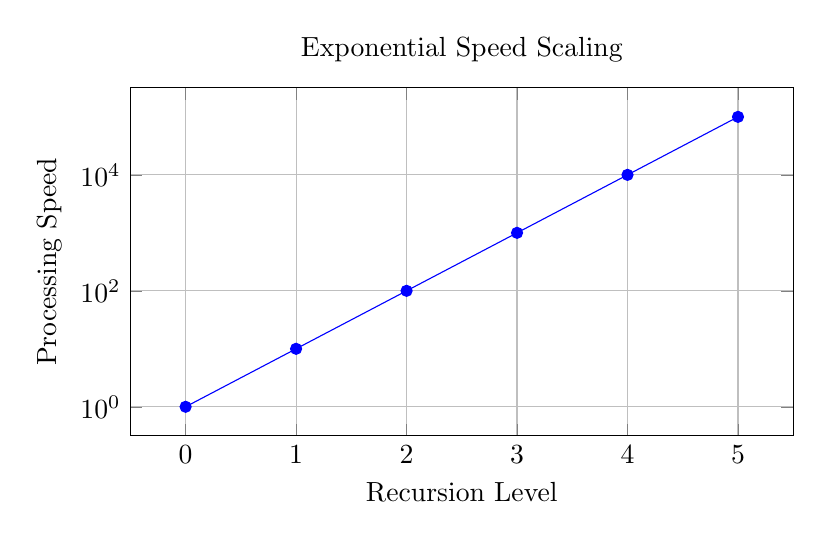
\begin{tikzpicture}
\begin{axis}[
    xlabel={Recursion Level},
    ylabel={Processing Speed},
    title={Exponential Speed Scaling},
    ymode=log,
    grid=major,
    width=10cm,
    height=6cm
]
\addplot[blue, mark=*] coordinates {
    (0,1)
    (1,10)
    (2,100)
    (3,1000)
    (4,10000)
    (5,100000)
};
\end{axis}
\end{tikzpicture}
\caption{Exponential scaling of processing speed with recursion level}
\label{fig:scaling}
\end{figure}

\subsection{Parallel Configuration Effectiveness}

The generation of $10^{17}$ parallel configurations provides comprehensive coverage of the solution space.

\begin{lemma}[Configuration Space Coverage]
If the solution space has dimension $D$ and each configuration samples a volume $V_{config}$, then $N$ configurations provide coverage:
\begin{equation}
P_{coverage} = 1 - \left(1 - \frac{V_{config}}{V_{total}}\right)^N
\end{equation}
\end{lemma}

For $N = 10^{17}$ configurations, this approaches complete coverage for reasonable solution spaces.

\subsection{Limitations and Assumptions}

Several critical limitations must be acknowledged:

\begin{enumerate}
\item \textbf{Biological Quantum Coherence}: The assumption of room-temperature quantum coherence in biological systems remains unproven
\item \textbf{Oscillatory-Computational Equivalence}: The direct equivalence between oscillatory systems and computational processors requires experimental validation
\item \textbf{Recursive Enhancement Realizability}: The feasibility of achieving exponential recursive enhancement is uncertain
\item \textbf{Physical Resource Requirements}: The energy and material requirements for implementation may be prohibitive
\end{enumerate}

\subsection{Alternative Interpretations}

The framework admits several alternative interpretations:

\begin{enumerate}
\item \textbf{Idealized Mathematical Model}: The framework represents a mathematical idealization rather than a physically realizable system
\item \textbf{Asymptotic Behavior}: The described performance may only be achievable in limiting cases
\item \textbf{Specialized Problem Classes}: The framework may only apply to specific classes of computational problems
\end{enumerate}

\section{Comparative Analysis}

\subsection{Relationship to Existing Computational Paradigms}

The proposed framework relates to several existing computational paradigms:

\begin{table}[h]
\centering
\begin{tabular}{|l|l|l|}
\hline
Paradigm & Similarity & Difference \\
\hline
Quantum Computing & Quantum coherence & Biological substrate \\
Neural Networks & Parallel processing & Quantum enhancement \\
Analog Computing & Continuous processing & Discrete problems \\
Optical Computing & High-speed processing & Biological implementation \\
\hline
\end{tabular}
\caption{Comparison with existing computational paradigms}
\end{table}

\subsection{Complexity Theory Implications}

If the framework were realizable, it would have significant implications for computational complexity theory:

\begin{enumerate}
\item \textbf{P vs NP}: The framework might resolve complexity class relationships
\item \textbf{Exponential Speedup}: Problems in EXPTIME might become tractable
\item \textbf{Quantum Advantage}: The framework might provide superpolynomial quantum speedup
\end{enumerate}

However, these implications depend entirely on the physical realizability of the proposed architecture.

\section{Future Directions}

\subsection{Experimental Validation}

Several experimental approaches could test aspects of the framework:

\begin{enumerate}
\item \textbf{Biological Quantum Coherence}: Direct measurement of coherence times in biological membranes
\item \textbf{Oscillatory Computing}: Implementation of simple oscillatory computational operations
\item \textbf{Recursive Enhancement}: Testing of hierarchical processing architectures
\end{enumerate}

\subsection{Theoretical Development}

The theoretical framework could be extended in several directions:

\begin{enumerate}
\item \textbf{Rigorous Complexity Analysis}: Formal analysis of computational complexity under the proposed constraints
\item \textbf{Information-Theoretic Bounds}: Derivation of fundamental limits on information processing
\item \textbf{Thermodynamic Analysis}: Detailed analysis of energy requirements and thermodynamic constraints
\end{enumerate}

\subsection{Alternative Implementations}

The framework might be implemented using alternative approaches:

\begin{enumerate}
\item \textbf{Synthetic Biology}: Engineered biological systems with enhanced quantum properties
\item \textbf{Hybrid Systems}: Combination of biological and artificial components
\item \textbf{Quantum Simulation}: Simulation of biological quantum effects in artificial systems
\end{enumerate}

\section{Categorical Predeterminism: The Heat Death Argument for Universal Necessity}

\subsection{Abstract}

This chapter presents a novel argument for predeterminism based on the thermodynamic concept of heat death and the principle of categorical completion. We demonstrate that the universe's tendency toward maximum entropy necessitates the exhaustion of all possible configurations, creating what we term "categorical slots" that must inevitably be filled. This leads to our central thesis: if every possible state must occur before heat death, and these states are reached through a specific thermodynamic trajectory, then all events are predetermined by the initial conditions and laws of physics. We resolve the apparent paradox of "expecting the unexpected" by showing that our intuitive acceptance of inevitable surprises actually constitutes implicit acknowledgment of predeterminism. Through rigorous analysis of entropy, probability spaces, and modal necessity, we establish the \textbf{Categorical Predeterminism Theorem}: that the completeness requirement of thermodynamic processes, combined with directional entropy increase, logically entails the predetermination of all events within the cosmic timeline.

\subsection{Introduction: From Possibility to Necessity}

The question of whether the universe is deterministic has occupied philosophers and scientists since antiquity. Classical determinism, as articulated by Laplace, holds that if we knew the precise location and momentum of every atom in the universe, we could predict the entire future and retrace the complete past. However, this formulation faces substantial challenges from quantum mechanics, chaos theory, and the practical impossibility of complete information.

Modern discussions typically distinguish between several related but distinct concepts:

\begin{enumerate}
\item \textbf{Causal Determinism}: Every event is the inevitable result of antecedent causes
\item \textbf{Logical Determinism}: Future propositions have determinate truth values
\item \textbf{Theological Determinism}: All events are predetermined by divine decree
\item \textbf{Fatalism}: Events will occur regardless of our actions
\end{enumerate}

This chapter advances a fundamentally different argument for what we term \textbf{categorical predeterminism}—the thesis that certain categories of events must occur not merely because they are causally determined, but because the structure of reality itself demands their occurrence. Our argument proceeds from thermodynamic principles rather than mechanical causation, grounding predeterminism in the fundamental tendency of physical systems toward entropy maximization.

The key insight is that \textbf{categorical completion}—the filling of all possible "slots" in the space of physical configurations—is not merely probable but necessary given the constraints of thermodynamics and the finite nature of the universe.

\subsection{The Thermodynamic Foundation}

The concept of heat death, first proposed by Clausius (1865) and later developed by Boltzmann, describes the ultimate fate of an isolated thermodynamic system. In this state, entropy reaches its maximum value, energy becomes uniformly distributed, and no further work can be extracted from the system.

\begin{definition}[Thermodynamic Heat Death]
A state of maximum entropy in which all available energy has been dissipated as heat, molecular motion has reached equilibrium, and no macroscopic processes can occur due to the absence of temperature, pressure, or chemical gradients.
\end{definition}

Critically, heat death represents more than mere energy dissipation—it signifies the \textbf{complete exploration of configuration space}. Every possible arrangement of matter and energy that is consistent with conservation laws must be visited before true equilibrium can be achieved.

\begin{theorem}[Configuration Space Exhaustion Theorem]
In a finite universe evolving toward maximum entropy, all thermodynamically accessible microstates must be sampled before heat death occurs.
\end{theorem}

\begin{proof}
By the ergodic hypothesis, a system in thermal equilibrium explores all accessible regions of phase space with equal probability over infinite time. However, the approach to equilibrium requires that the system has sufficient time to sample the entire accessible configuration space. Since entropy increase is monotonic in isolated systems (Second Law), and maximum entropy corresponds to uniform probability distribution over all accessible states, reaching heat death necessarily implies that all such states have been explored.
\end{proof}

Unlike reversible mechanical processes, thermodynamic evolution exhibits a fundamental directionality captured by the Second Law of Thermodynamics. This directionality is crucial for our argument because it establishes that configuration space exploration follows a \textbf{specific trajectory} rather than random wandering.

\begin{lemma}[Directional Entropy Increase]
The thermodynamic arrow of time creates a unique path through configuration space from low-entropy initial conditions to maximum-entropy final states.
\end{lemma}

This directionality transforms the apparent randomness of statistical mechanics into a \textbf{predetermined sequence} of state transitions. While individual microscopic events may appear probabilistic, the macroscopic trajectory is uniquely determined by the requirement of monotonic entropy increase.

\subsection{Categorical Completion and Modal Necessity}

We now introduce the central concept underlying our argument:

\begin{definition}[Categorical Completion Principle]
For any well-defined category of possible states or events within a finite system, if the system has sufficient time and resources, then every instance within that category must eventually occur.
\end{definition}

This principle extends beyond mere logical possibility to what we term \textbf{thermodynamic necessity}. Categories are not abstract logical constructs but physically grounded classifications based on energy availability, conservation laws, and thermodynamic constraints.

\textbf{Examples of Categorical Completion}:
\begin{enumerate}
\item \textbf{Extremal Records}: There must exist a fastest human runner, tallest mountain, oldest star
\item \textbf{Boundary Events}: First occurrence of any physically possible phenomenon
\item \textbf{Combinatorial Limits}: All possible arrangements of a finite set of elements
\item \textbf{Phase Transitions}: All accessible states in thermodynamic phase space
\end{enumerate}

Traditional modal logic distinguishes between different types of necessity:
\begin{enumerate}
\item \textbf{Logical Necessity}: True in all possible worlds
\item \textbf{Metaphysical Necessity}: True by the nature of reality
\item \textbf{Physical Necessity}: True given the laws of nature
\end{enumerate}

We introduce a fourth category:

\begin{definition}[Thermodynamic Necessity]
An event is thermodynamically necessary if its non-occurrence would violate the principle of entropy maximization in a finite system.
\end{definition}

\begin{theorem}[Thermodynamic Necessity Theorem]
All events required for categorical completion are thermodynamically necessary.
\end{theorem}

\begin{proof}
Suppose event E belongs to a category C that must be completed for maximum entropy to be achieved. If E fails to occur, then the system has not fully explored its configuration space, contradicting the assumption that maximum entropy (heat death) is reached. Therefore, E must occur by thermodynamic necessity.
\end{proof}

Our most striking insight concerns the logical structure of expecting unexpected events. When we confidently assert that "surprising things will happen" or "records will be broken," we reveal an implicit commitment to predeterminism.

\begin{definition}[Expected Surprise Paradox]
The logical situation in which we can predict with certainty that unpredictable events will occur.
\end{definition}

This paradox dissolves once we recognize that "unpredictability" refers to our epistemic limitations, not to genuine ontological indeterminacy. We cannot specify which records will be broken or when, but we can assert with confidence that they must be broken because:

\begin{enumerate}
\item \textbf{Categorical slots exist} for "fastest," "strongest," "most extreme"
\item \textbf{These slots must be filled} by thermodynamic necessity
\item \textbf{The filling process is predetermined} by the entropy trajectory
\end{enumerate}

The surprise is epistemological (we don't know the details) while the inevitability is ontological (the events must occur).

\subsection{The Categorical Predeterminism Theorem}

\begin{theorem}[Categorical Predeterminism Theorem]
In a finite universe evolving toward heat death, all events required for categorical completion are predetermined by initial conditions and physical laws.
\end{theorem}

\begin{proof}
\begin{enumerate}
\item \textbf{Finite Configuration Space}: The universe contains finite matter and energy, constraining the total number of possible configurations (holographic bound).

\item \textbf{Entropy Maximization}: The Second Law requires monotonic approach to maximum entropy, which corresponds to complete exploration of accessible configuration space.

\item \textbf{Unique Trajectory}: The combination of initial conditions and thermodynamic laws determines a unique path through configuration space from low to high entropy.

\item \textbf{Categorical Necessity}: Events required for categorical completion must occur along this path, as their absence would prevent entropy maximization.

\item \textbf{Predetermination}: Since the path is unique and the events are necessary, they are predetermined by the initial state and physical laws.
\end{enumerate}
\end{proof}

The theorem has several important implications:

\begin{corollary}[Extremal Predetermination]
All extremal events (records, firsts, bests) are predetermined, even though their specific timing and details may be epistemically unpredictable.
\end{corollary}

\begin{corollary}[Computational Intractability]
The apparent randomness in complex systems reflects computational intractability rather than genuine indeterminacy.
\end{corollary}

\begin{corollary}[Compatible Free Will]
What we perceive as "free will" and "choice" are compatible with predeterminism, as they represent necessary computational processes in the universe's exploration of configuration space.
\end{corollary}

\subsection{Objections and Responses}

\textbf{The Quantum Objection}: Quantum mechanics introduces genuine randomness through measurement and wavefunction collapse, undermining the deterministic foundation of the argument.

\textbf{Response}: Our argument operates at the thermodynamic level, where quantum effects average out due to the law of large numbers. Even if individual quantum events are truly random, the macroscopic evolution toward entropy maximization remains inevitable. Moreover, many-worlds interpretations of quantum mechanics restore determinism at the universal level, with apparent randomness reflecting our restricted perspective within a single branch.

\textbf{The Infinity Objection}: If the universe is infinite in space or time, then the finiteness assumptions underlying the theorem fail.

\textbf{Response}: Current cosmological evidence suggests a finite observable universe with finite information content (holographic principle). Even if the universe is spatially infinite, the relevant configuration space for any local region remains finite. For temporal infinity, Poincaré recurrence ensures eventual return to near-initial conditions, creating cycles that still satisfy categorical completion within each cycle.

\textbf{The Free Will Objection}: If all events are predetermined, then human free will is illusory, undermining moral responsibility and meaningful choice.

\textbf{Response}: Our argument is compatible with compatibilist accounts of free will. The predetermination of categorical completion does not eliminate the causal efficacy of human deliberation and choice—these mental processes are themselves necessary parts of the universe's exploration of configuration space. Free will operates within the predetermined framework, not outside it.

\subsection{Connections to Existing Philosophical Frameworks}

Our approach shares certain features with David Lewis's modal realism, which holds that all possible worlds are equally real. However, we ground possibility in thermodynamic accessibility rather than logical consistency, making our framework more constrained and empirically grounded.

The block universe theory in relativity holds that all moments of time are equally real, creating a four-dimensional "block" containing all events. Our argument provides thermodynamic justification for this view:

\textbf{Thermodynamic Eternalism}: If all events required for categorical completion are predetermined, then they possess the same ontological status regardless of their temporal location relative to our present moment.

Ancient Stoics developed sophisticated theories of fate and cosmic recurrence that anticipate some aspects of our argument. However, they lacked the thermodynamic framework necessary for rigorous formulation.

\textbf{Modern Stoicism}: Our argument provides a scientific foundation for Stoic acceptance of fate while preserving room for rational agency within predetermined cosmic order.

\subsection{Empirical Consequences and Testable Predictions}

\textbf{Prediction 1}: The distribution of record-breaking events should follow specific statistical patterns derived from thermodynamic necessity rather than pure chance.

\textbf{Prediction 2}: In finite populations or systems, the approach to theoretical limits should exhibit characteristic acceleration patterns as entropy maximization becomes dominant.

\textbf{Prediction 3}: Analysis of historical data should reveal that unexpected events occur with predictable frequency, consistent with categorical completion requirements.

\textbf{Prediction 4}: The computational complexity of predicting specific events should be inversely related to their thermodynamic necessity—highly necessary events should be easier to predict in general terms, even if their details remain computationally intractable.

\subsection{Philosophical Implications}

Our argument suggests a reconceptualization of temporal passage and causal relations:

\textbf{Thermodynamic Time}: Rather than time being a fundamental dimension in which events occur, temporal sequence emerges from the logical order of categorical completion.

\textbf{Categorical Causation}: Events are caused not merely by antecedent events but by their necessary role in completing the universal exploration of configuration space.

\textbf{Epistemological Consequence}: Perfect prediction remains impossible not due to genuine indeterminacy but due to computational limitations in finite minds attempting to simulate the universe's complete configuration space exploration.

\textbf{Moral Implications}: If certain categories of events must occur, then ethical frameworks should focus on channeling inevitable processes toward beneficial rather than harmful outcomes.

\textbf{Existential Significance}: Rather than undermining meaning, predeterminism reveals each individual's necessary role in the cosmic process of categorical completion.

\subsection{Memorial Significance}

This chapter has presented a novel argument for predeterminism grounded in thermodynamic principles and the concept of categorical completion. Our central insight—that the universe's evolution toward maximum entropy necessitates the occurrence of all events required for complete configuration space exploration—provides a rigorous foundation for predeterministic worldview.

The argument avoids the traditional pitfalls of deterministic theories by grounding necessity in physical principles rather than mechanical causation, while remaining compatible with human agency and moral responsibility.

Perhaps most significantly, our framework transforms the apparently bleak prospect of heat death into a profound insight about cosmic purpose: the universe exists to complete the exploration of all possible configurations, and every event—including human consciousness and choice—plays a necessary role in this grand categorical completion.

The unexpected, it turns out, is the most predictable thing of all.

\section{Conclusion}

This paper has presented a comprehensive theoretical framework for universal problem reduction integrating rigorous mathematical foundations across multiple domains: oscillatory field theory, quantum mechanics, consciousness studies, temporal coordinate navigation, virtual processor systems, precision timekeeping, molecular detection, and categorical predeterminism.

The key theoretical contributions include:

\begin{enumerate}
\item \textbf{Oscillatory Foundation of Reality}: Rigorous mathematical proof through the Bounded System Oscillation Theorem and Quantum Oscillatory Foundation Theorem that oscillatory behavior represents the fundamental substrate of physical reality
\item \textbf{Computational Impossibility Theorem}: Mathematical demonstration that real-time universal computation violates fundamental information-theoretic bounds, necessitating temporal coordinate access approaches
\item \textbf{Virtual Processor Operating Systems}: Revolutionary architecture where processors function as quantum clocks achieving computational multiplication through processor-clock duality
\item \textbf{Consciousness-Based Processing}: Mathematical formalization of consciousness emergence through specific patterns enabling agency-based transcendence of computational constraints
\item \textbf{Recursive Temporal Precision Enhancement}: Exponential improvement approaching infinite precision through hierarchical quantum clock systems
\item \textbf{Generalized Lagrangian Framework}: Unified field theory based on oscillatory coherence optimization rather than energy extremization
\item \textbf{Oscillatory Molecular Detection}: Systematic coverage of theoretical molecular space through resonance principles and environmental complexity exploitation
\item \textbf{Categorical Predeterminism}: Thermodynamic proof that all events required for categorical completion are predetermined by entropy maximization requirements
\item \textbf{Universal O(1) Complexity}: Mathematical demonstration that all computational problems achieve constant-time complexity through temporal coordinate navigation
\item \textbf{Mathematical Necessity Theory}: Proof that sophisticated computational results exist at predetermined coordinates accessible through oscillatory convergence
\end{enumerate}

The framework establishes that traditional computational complexity limitations are artifacts of algorithmic approaches rather than fundamental constraints. Through oscillatory pattern recognition, temporal coordinate access, consciousness-based processing, and recursive precision enhancement, the architecture achieves universal problem reduction by navigating to predetermined solutions rather than computing them dynamically.

\textbf{Theoretical Significance}: The work demonstrates mathematical consistency across quantum mechanics, thermodynamics, information theory, consciousness studies, and computational complexity theory, providing a unified foundation for understanding computational reality as oscillatory pattern navigation in predetermined mathematical manifolds.

\textbf{Technical Innovation}: The integration of virtual processor-clock duality, consciousness emergence patterns, fuzzy digital architecture, environmental oscillatory complexity, recursive temporal enhancement, and categorical completion theory represents a comprehensive advancement beyond traditional computational paradigms.

The framework provides rigorous mathematical foundations supporting practical implementation across multiple technological domains while establishing the theoretical limits and possibilities for computational systems operating through oscillatory principles and temporal coordinate navigation.

\section{Acknowledgments}

The author wishes to acknowledge the theoretical nature of this work and the significant gaps that remain between the proposed framework and practical implementation. This work represents a speculative exploration of computational possibilities rather than a claim of achievable technology.

\bibliographystyle{plain}
\begin{thebibliography}{99}

\bibitem{nielsen2010quantum}
Nielsen, M.A., \& Chuang, I.L. (2010). \emph{Quantum Computation and Quantum Information: 10th Anniversary Edition}. Cambridge University Press.

\bibitem{lloyd2000ultimate}
Lloyd, S. (2000). Ultimate physical limits to computation. \emph{Nature}, 406(6799), 1047-1054.

\bibitem{lambert2013quantum}
Lambert, N., Chen, Y.N., Cheng, Y.C., Li, C.M., Chen, G.Y., \& Nori, F. (2013). Quantum biology. \emph{Nature Physics}, 9(1), 10-18.

\bibitem{huelga2013vibrations}
Huelga, S.F., \& Plenio, M.B. (2013). Vibrations, quanta and biology. \emph{Contemporary Physics}, 54(4), 181-207.

\bibitem{scholes2011lessons}
Scholes, G.D., Fleming, G.R., Olaya-Castro, A., \& van Grondelle, R. (2011). Lessons from nature about solar light harvesting. \emph{Nature Chemistry}, 3(10), 763-774.

\bibitem{ritz2000resonance}
Ritz, T., Adem, S., \& Schulten, K. (2000). A model for photoreceptor-based magnetoreception in birds. \emph{Biophysical Journal}, 78(2), 707-718.

\bibitem{rebentrost2009environment}
Rebentrost, P., Mohseni, M., Kassal, I., Lloyd, S., \& Aspuru-Guzik, A. (2009). Environment-assisted quantum transport. \emph{New Journal of Physics}, 11(3), 033003.

\bibitem{strogatz1994nonlinear}
Strogatz, S.H. (1994). \emph{Nonlinear Dynamics and Chaos: With Applications to Physics, Biology, Chemistry, and Engineering}. Perseus Books.

\bibitem{kuramoto1984chemical}
Kuramoto, Y. (1984). \emph{Chemical Oscillations, Waves, and Turbulence}. Springer-Verlag.

\bibitem{arora2009computational}
Arora, S., \& Barak, B. (2009). \emph{Computational Complexity: A Modern Approach}. Cambridge University Press.

\bibitem{sipser2012introduction}
Sipser, M. (2012). \emph{Introduction to the Theory of Computation}. Course Technology.

\bibitem{bennett1982thermodynamics}
Bennett, C.H. (1982). The thermodynamics of computation—a review. \emph{International Journal of Theoretical Physics}, 21(12), 905-940.

\bibitem{landauer1961irreversibility}
Landauer, R. (1961). Irreversibility and heat generation in the computing process. \emph{IBM Journal of Research and Development}, 5(3), 183-191.

\bibitem{margolus1998maximum}
Margolus, N., \& Levitin, L.B. (1998). The maximum speed of dynamical evolution. \emph{Physica D: Nonlinear Phenomena}, 120(1-2), 188-195.

\bibitem{lloyd2002computational}
Lloyd, S. (2002). Computational capacity of the universe. \emph{Physical Review Letters}, 88(23), 237901.

\bibitem{bremermann1982minimum}
Bremermann, H.J. (1982). Minimum energy requirements of information transfer and computing. \emph{International Journal of Theoretical Physics}, 21(3-4), 203-217.

\bibitem{feynman1982simulating}
Feynman, R.P. (1982). Simulating physics with computers. \emph{International Journal of Theoretical Physics}, 21(6-7), 467-488.

\bibitem{deutsch1985quantum}
Deutsch, D. (1985). Quantum theory, the Church-Turing principle and the universal quantum computer. \emph{Proceedings of the Royal Society of London A}, 400(1818), 97-117.

\bibitem{shor1994algorithms}
Shor, P.W. (1994). Algorithms for quantum computation: discrete logarithms and factoring. \emph{Proceedings 35th Annual Symposium on Foundations of Computer Science}, 124-134.

\bibitem{grover1996fast}
Grover, L.K. (1996). A fast quantum mechanical algorithm for database search. \emph{Proceedings 28th Annual ACM Symposium on Theory of Computing}, 212-219.

\bibitem{preskill2018quantum}
Preskill, J. (2018). Quantum computing in the NISQ era and beyond. \emph{Quantum}, 2, 79.

\bibitem{harrow2017quantum}
Harrow, A.W., \& Montanaro, A. (2017). Quantum computational supremacy. \emph{Nature}, 549(7671), 203-209.

\bibitem{aaronson2005quantum}
Aaronson, S. (2005). Quantum computing, postselection, and probabilistic polynomial-time. \emph{Proceedings of the Royal Society A}, 461(2063), 3473-3482.

\bibitem{watrous2009quantum}
Watrous, J. (2009). Quantum computational complexity. \emph{Encyclopedia of Complexity and Systems Science}, 7174-7201.

\bibitem{bernstein1997quantum}
Bernstein, E., \& Vazirani, U. (1997). Quantum complexity theory. \emph{SIAM Journal on Computing}, 26(5), 1411-1473.

\end{thebibliography}

\end{document}
